\chapter{HASIL DAN PEMBAHASAN}
Pada subbab pertama pada bab ini akan dipaparkan hasil akhir dari pengerjaan tugas akhir Interoperabilitas NFT Berbasis \emph{Blockchain} Menggunakan \emph{Smart Contract} pada WEB3.0. Pada subbab selanjutnya akan dipaparkan mengenai hasil pengujian dari hasil tugas akhir untuk memastikan bahwa sistem yang dikembangkan berjalan dengan sesuai.

\section{Hasil}
Hasil keseluruhan dari sistem yang dikembangkan adalah \emph{interface} berupa web, \emph{Non-Fungible Token} (NFT) dan juga \emph{smart contract} yang berinteroperabilitas. Berikut dipaparkan masing-masing hasil dari sistem yang dikembangkan.

\subsection{Web Interface}
Tampilan awal web \emph{interface}, menampilkan daftar koleksi NFT yang dapat di-\emph{minting}. Nantinya NFT tersebut dapat dimiliki oleh \emph{address} yang melakukan pertama kali \emph{minting} dan juga kepemilikan dari NFT tersebut dapat diberikan ke \emph{address} lain.
\begin{figure} [H] \centering
  % Nama dari file gambar yang diinputkan
  \frame{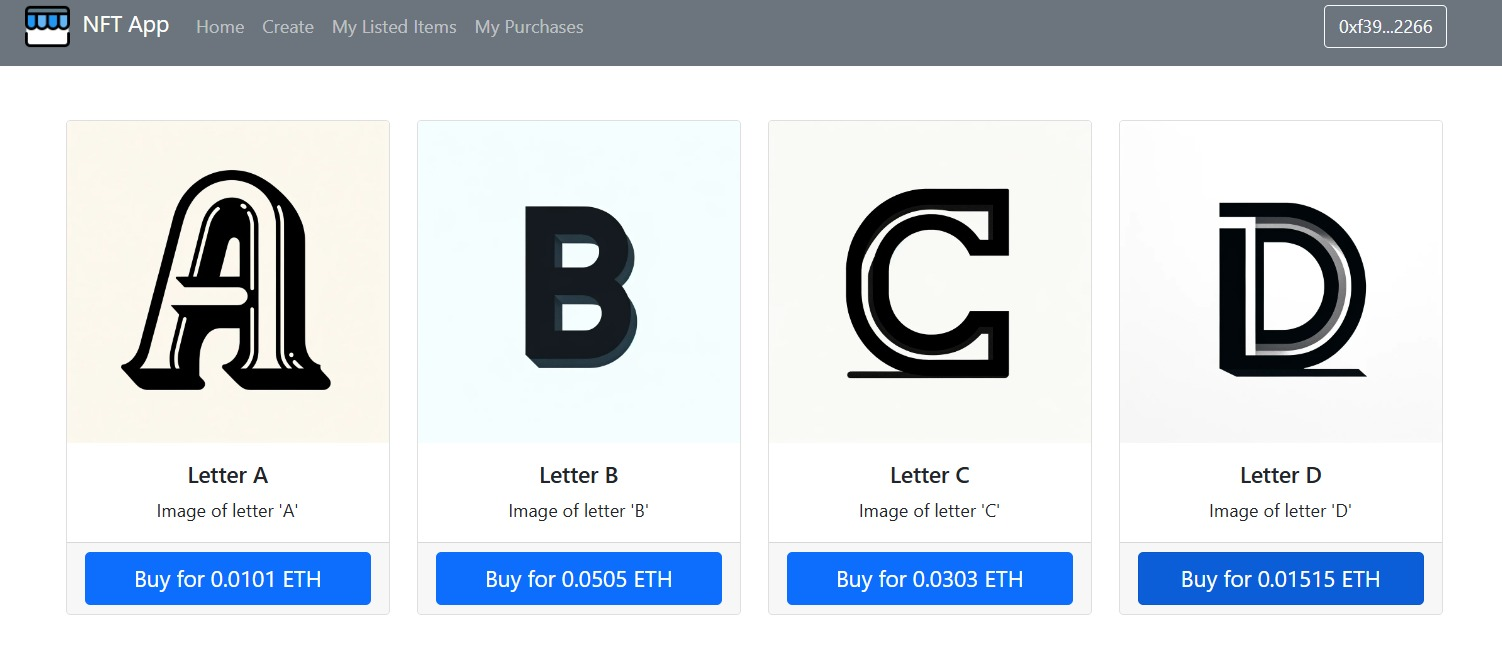
\includegraphics[scale=0.30]{gambar/tampilan_aplikasi.jpeg}}
  % Keterangan gambar yang diinputkan
  \caption{Tampilan interface}
  % Label referensi dari gambar yang diinputkan
  \label{fig:interface}
\end{figure}

Pada halaman dashboard awal, pengguna diharuskan untuk menekan tombol Connect Wallet, yang akan memicu proses koneksi dengan Metamask Wallet. Setelah berhasil terhubung, pengguna akan mendapatkan address yang bersifat unik. Alamat ini tidak hanya penting untuk keperluan identifikasi pengguna di dalam jaringan, tetapi juga berfungsi sebagai kunci akses untuk melakukan minting token NFT. Dengan demikian, address tersebut menjadi sangat krusial karena merupakan representasi digital dari identitas pengguna dalam ekosistem blockchain, memungkinkan mereka untuk bertransaksi, mengakses, dan mengelola aset digital mereka dengan aman. Proses ini memastikan bahwa setiap interaksi yang dilakukan melalui smart contract untuk NFT tercatat secara transparan dan dapat diverifikasi, memberikan keamanan dan kepercayaan dalam setiap transaksi.

  \begin{figure} [H] \centering
  % Nama dari file gambar yang diinputkan
  \frame{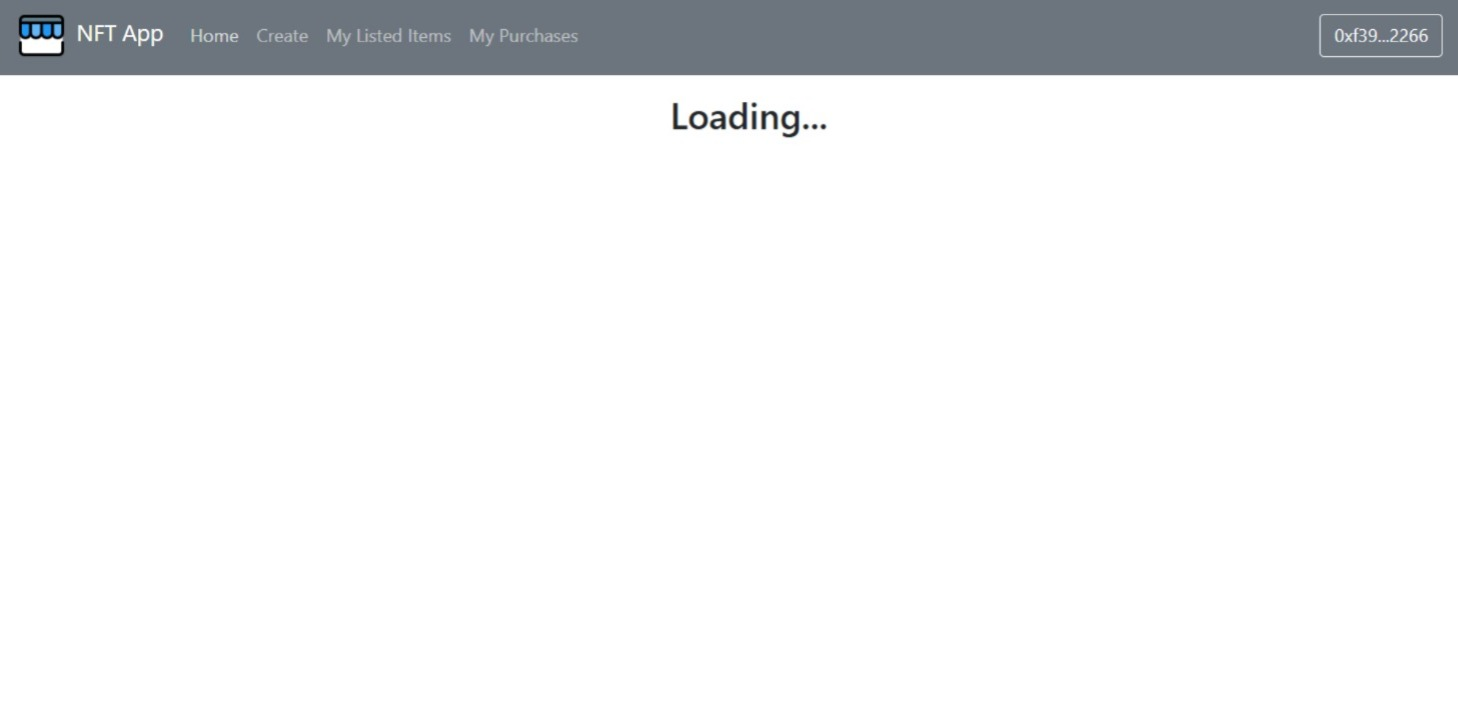
\includegraphics[scale=0.27]{gambar/home_page.jpg}}
  % Keterangan gambar yang diinputkan
  \caption{Tampilan awal dari web}
  % Label referensi dari gambar yang diinputkan
  \label{fig:homepage}
  \end{figure}

  Pada gambar \ref{fig:homepage} adalah tampilan dari \emph{homepage} awal ketika pengguna menekan tombol \emph{home} pada \emph{navigation bar} atas. Pada web ini terdapat beberapa halaman yang dapat diakses dengan menekan tombol pada \emph{navigation bar}, seperti \emph{Home}, \emph{Create}, \emph{My Listed Items}, dan \emph{My Purchase}. Tampilan-tampilan ini dapat diakses ketika pengguna telah melakukan koneksi web dengan Metamask Wallet, hal ini dapat dilihat pada \emph{navigation bar} atas kanan terdapat \emph{address} dari akun Metamask Wallet. Pada tampilan awal ini, pengguna dapat melihat NFT yang telah diunggah untuk dapat dilakukan pembelian atau \emph{minting}. Tetapi karena belum terdapat NFT yang diunggah maka hanya akan menampilkan tulisan "\emph{Loading...}".
   
  \begin{figure} [H] \centering
    % Nama dari file gambar yang diinputkan
    \frame{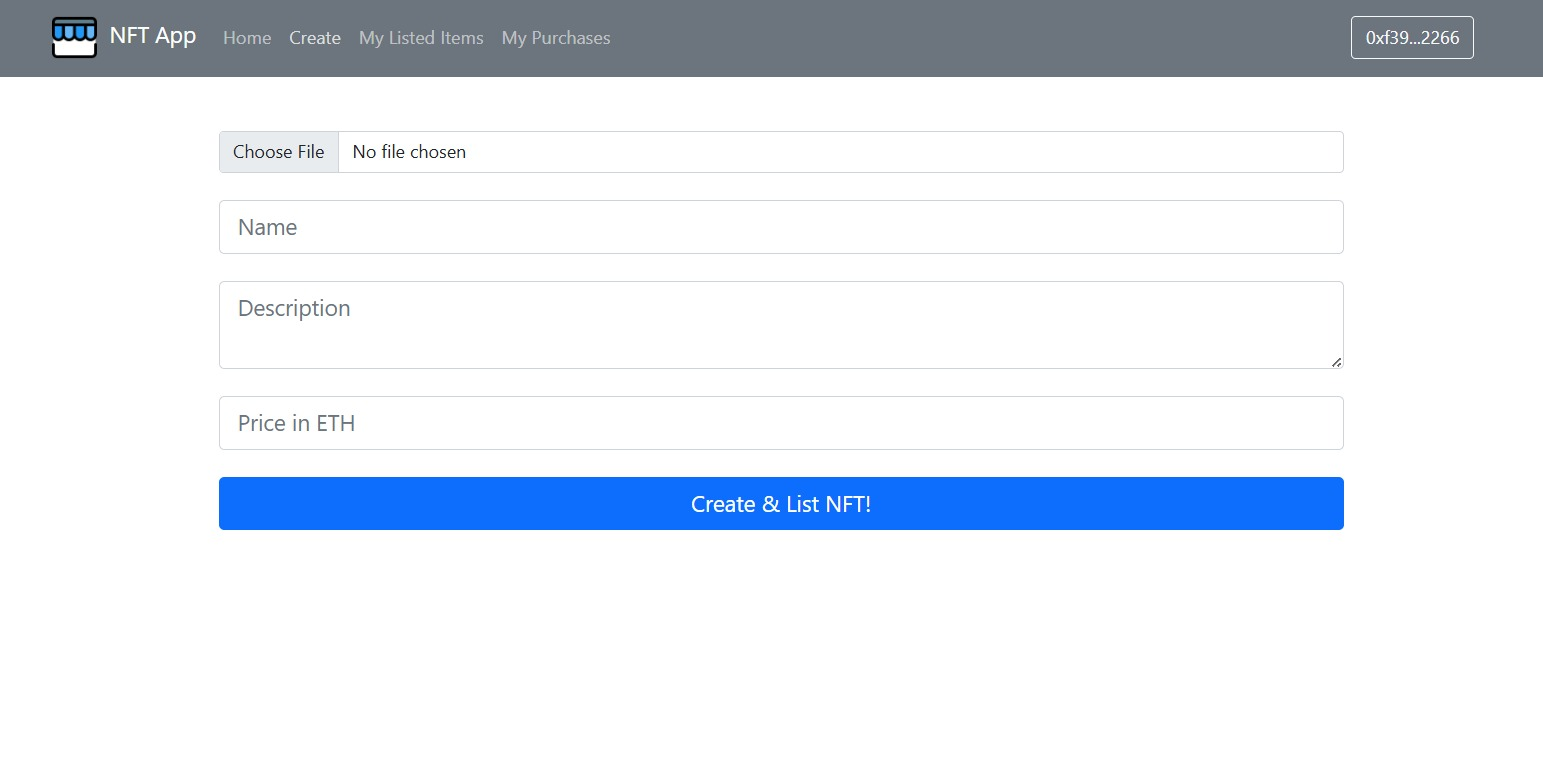
\includegraphics[scale=0.27]{gambar/create_page.jpeg}}
    % Keterangan gambar yang diinputkan
    \caption{Tampilan halaman \emph{create}}
    % Label referensi dari gambar yang diinputkan
    \label{fig:createpage}
    \end{figure}

  Pada gambar \ref{fig:createpage} adalah tampilan dari \emph{create page}. Pada halaman ini pengguna dapat mengunggah sebuah NFT berupa gambar ke web yang kemudian jika diunggah akan muncul pada halaman \emph{home} dan juga akan muncul pada halaman \emph{my listed items}.

  \begin{figure} [H] \centering
    % Nama dari file gambar yang diinputkan
    \frame{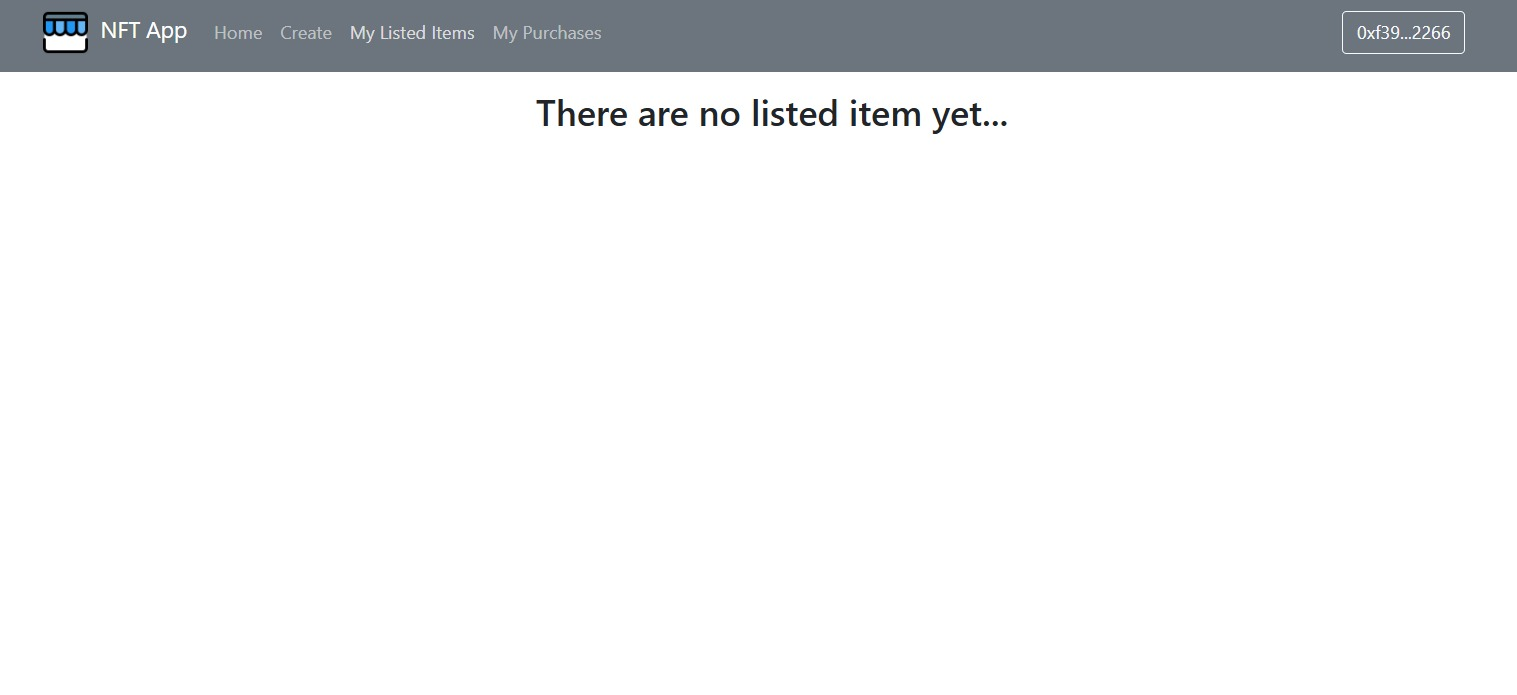
\includegraphics[scale=0.27]{gambar/listing_page.jpg}}
    % Keterangan gambar yang diinputkan
    \caption{Tampilan halaman \emph{my listed items}}
    % Label referensi dari gambar yang diinputkan
    \label{fig:listingpage}
    \end{figure}
  
  Pada gambar \ref{fig:listingpage} adalah tampilan dari \emph{my listed items page}. Pada halaman ini pengguna dapat melihat NFT kepemilikannya yang telah diunggah pada ketika dia melakukan \emph{create}. Tetapi dikarenakan belum melakukan pengunggahan NFT, maka halaman ini hanya akan memunculkan tulisan "\emph{There are no listed item yet}".

  \begin{figure} [H] \centering
    % Nama dari file gambar yang diinputkan
    \frame{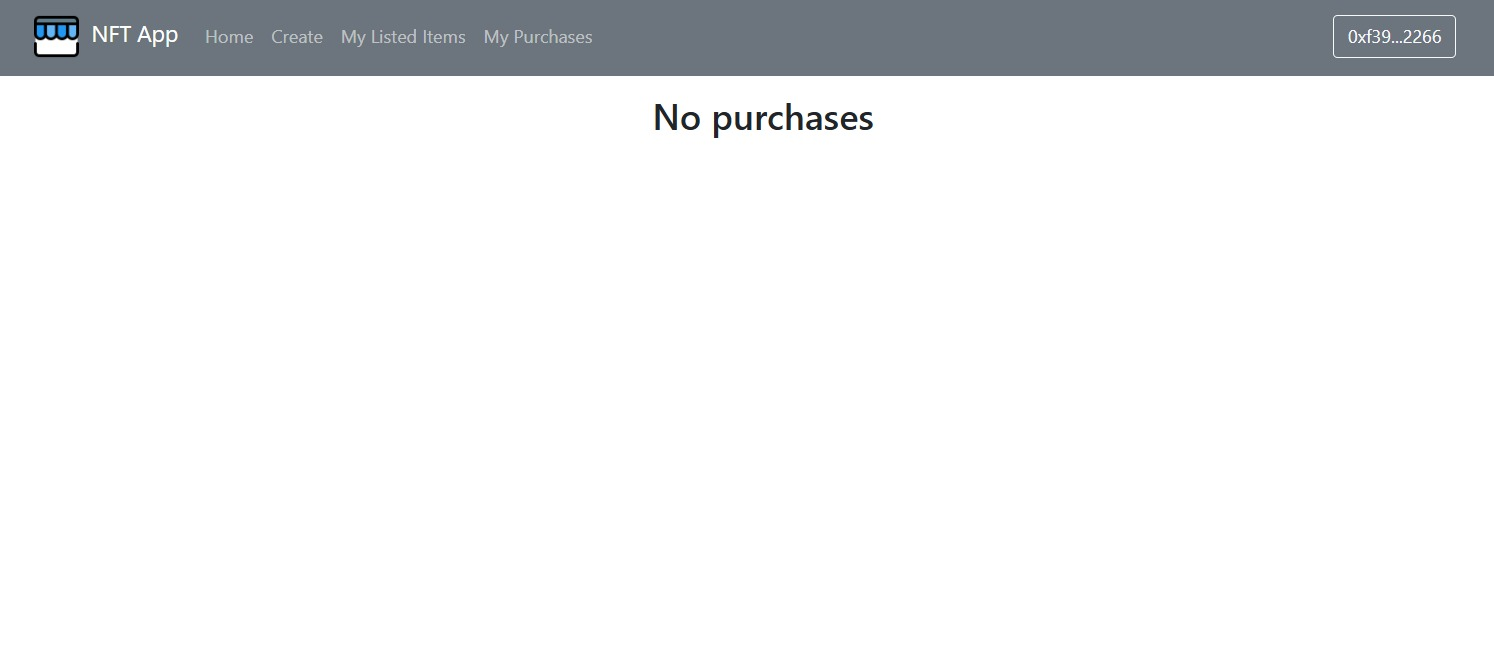
\includegraphics[scale=0.27]{gambar/purchase_page.jpg}}
    % Keterangan gambar yang diinputkan
    \caption{Tampilan halaman \emph{my purchases}}
    % Label referensi dari gambar yang diinputkan
    \label{fig:purchasepage}
    \end{figure}
  
  Pada gambar \ref{fig:purchasepage}, terlihat tampilan dari \emph{my purchase page} yang dirancang khusus untuk memungkinkan pengguna melihat semua NFT yang telah mereka peroleh melalui pembelian di halaman utama platform. Setelah melakukan pembelian, NFT tersebut akan terdaftar di halaman ini, memberikan tampilan visual serta detail dari setiap NFT yang dimiliki. Lebih lanjut, halaman ini juga menyediakan fungsi \emph{transfer ownership}, yang memungkinkan pemilik untuk mengalihkan kepemilikan NFT kepada pengguna lain dengan \emph{address} yang berbeda. Fungsi ini sangat penting untuk mendukung fleksibilitas dan likuiditas dalam perdagangan NFT di pasar. Namun, jika pengguna belum melakukan pembelian apapun, halaman ini akan menampilkan pesan "\emph{No purchases}", yang menandakan bahwa tidak ada NFT yang dapat ditampilkan atau ditransfer.z

\subsection{\emph{Smart Contract}}
Dalam pengembangan aplikasi berbasis \emph{blockchain}, pengintegrasian \emph{smart contract} dengan antarmuka pengguna seperti React.js menjadi krusial. \emph{Smart contract} yang dibangun menggunakan Solidity dapat di-\emph{deploy} di \emph{testnet} Ethereum, seperti Sepolia Testnet, yang menyediakan lingkungan yang hampir mirip dengan mainnet Ethereum namun tanpa memerlukan biaya transaksi yang besar. 

ABI atau \emph{Application Binary Interface}, adalah cara yang memungkinkan fungsi dalam \emph{smart contract} Ethereum untuk berkomunikasi dengan aplikasi eksternal, termasuk antarmuka pengguna yang dibangun dengan kerangka kerja seperti React.js. ABI berperan sebagai lapisan translasi yang menguraikan cara memanggil fungsi dalam smart contract, jenis parameter yang diterima, jenis keluaran yang diharapkan, serta sifat state dari fungsi tersebut. ABI biasanya dihasilkan secara otomatis oleh \emph{compiler} Solidity sebagai bagian dari proses kompilasi \emph{smart contract} dan disimpan dalam format JSON. Setiap kali aplikasi \emph{frontend} mengirimkan transaksi atau \emph{query} ke \emph{blockchain}, ia menggunakan ABI untuk mengkodekan data panggilan ke dalam format yang dapat dipahami oleh \emph{Ethereum Virtual Machine} (EVM). Kemudian, saat data dikembalikan dari \emph{smart contract}, ABI digunakan untuk mendekode balasan sehingga aplikasi React.js dapat memahami dan memprosesnya.

Proses \emph{deploy} dilakukan \emph{smart contract} akan di-\emph{deploy} ke beberapa jaringan \emph{blockchain} namun dikarenakan dalam pengujian ini yang digunakan adalah sepolia \emph{testnet} maka yang digunakan hanyalah dari jaringan sepolia \emph{testnet}. Ketika melakukan proses \emph{deployment} akan dikenakan \emph{gas} atau fee yang dapat dibayar menggunakan \emph{ethereum} yang terdapat pada \emph{wallet} Metamask. Yang kemudian detail dari transaksi tersebut dapat dilihat pada Etherscan.

\begin{figure} [H] \centering
  % Nama dari file gambar yang diinputkan
  \frame{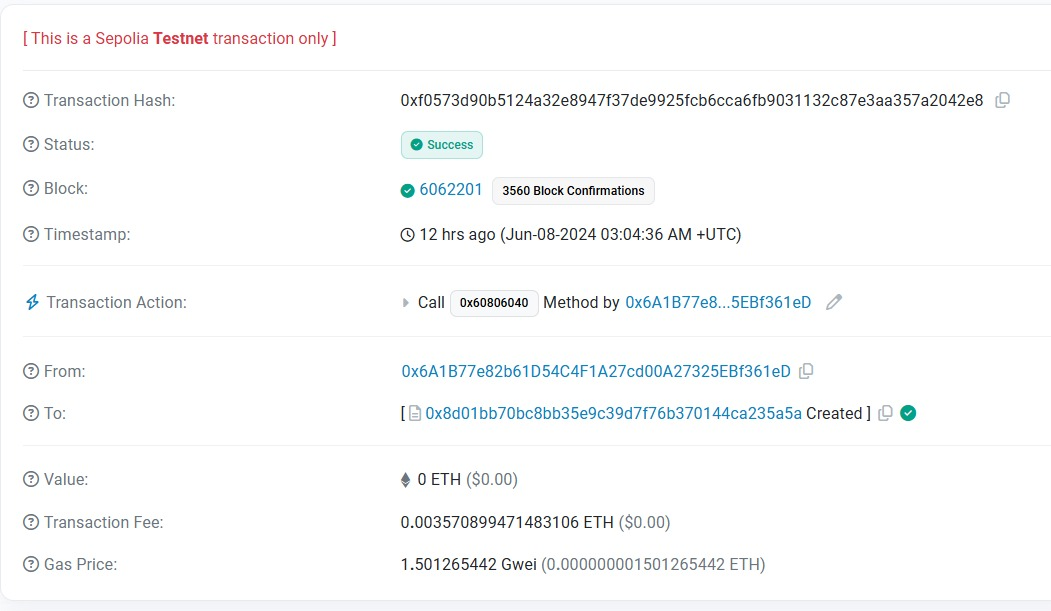
\includegraphics[scale=0.45]{gambar/etherscan.jpeg}}
  % Keterangan gambar yang diinputkan
  \caption{Detail transaksi pada etherscan}
  % Label referensi dari gambar yang diinputkan
  \label{fig:transaction}
\end{figure}

\subsection{\emph{Non-Fungible Token} (NFT)}
\emph{Non-Fungible Token} (NFT) sendiri juga memiliki beberapa tahapan agar dapat dapat disimpan dalam \emph{The Interplanetary File System} (IPFS) dan kemudian dapat di-\emph{publish} pada OpenSea \emph{test net}. Pada pengerjaan tugas akhir ini, Pinata digunakan sebagai \emph{platform} untuk mengunggah foto NFT dan juga data \emph{JavaScript Object Notation} (JSON) agar bisa di-\emph{minting} sebagai \emph{Uniform Resource Identifier} (URI) pada \emph{smart contract}. Hal ini dibutuhkan agar NFT yang di-\emph{minting} memiliki gambar yang dapat dilihat pada OpenSea.

\begin{figure} [H] \centering
  % Nama dari file gambar yang diinputkan
  \frame{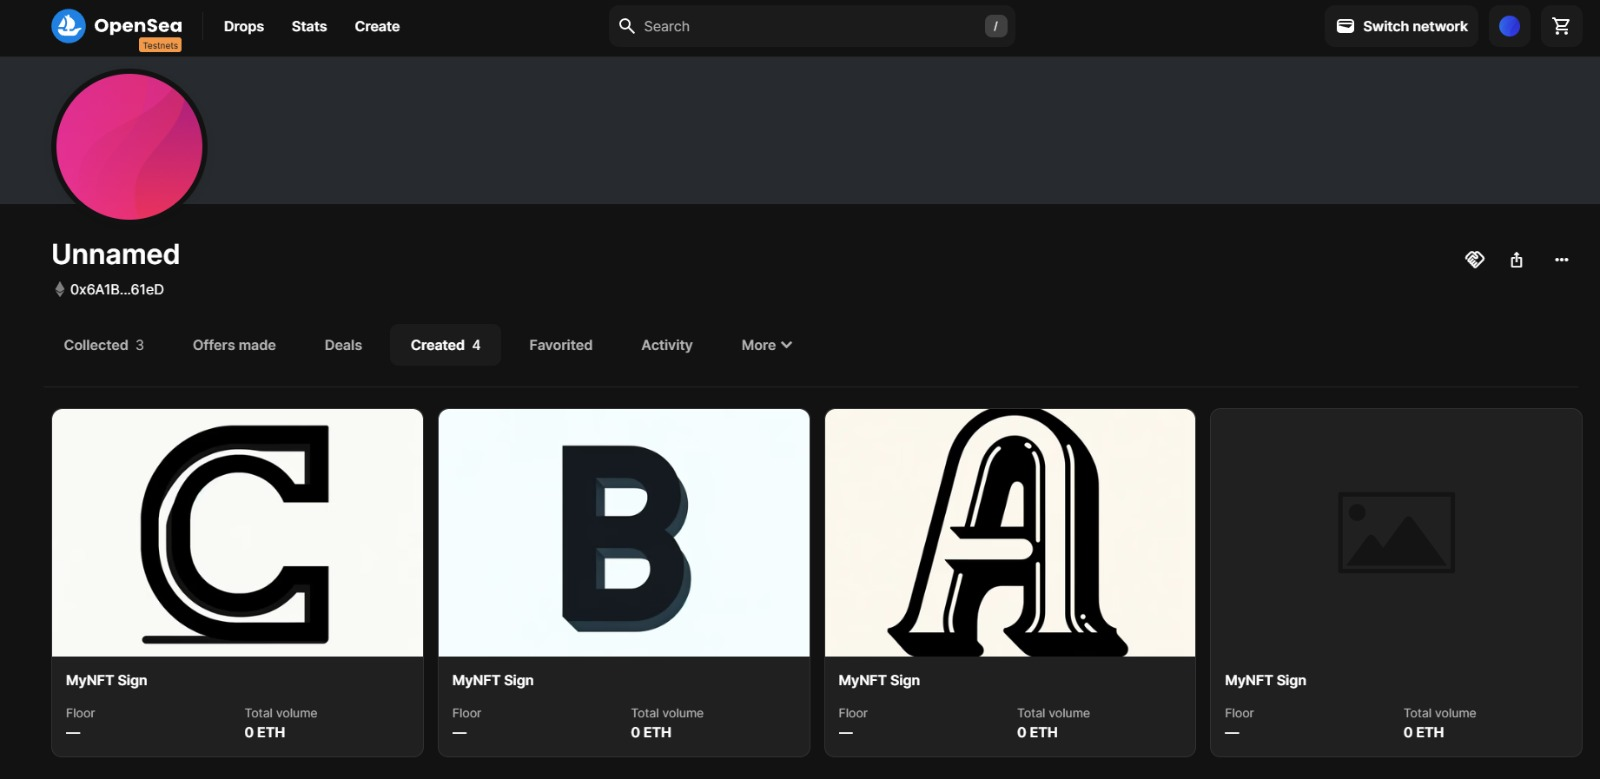
\includegraphics[scale=0.28]{gambar/opensea.jpeg}}
  % Keterangan gambar yang diinputkan
  \caption{NFT terunggah pada Opensea}
  % Label referensi dari gambar yang diinputkan
  \label{fig:opensea}
\end{figure}

\section{Pengujian}
Untuk memastikan bahwa sistem interoperabilitas \emph{Smart Contract} berjalan sesuai dengan yang direncakan maka perlu dilakukan pengujian lebih lanjut. Pengujian yang dilakukan secara garis besar dibagi menjadi dua yaitu Pengujian fitur-fitur utama dari \emph{Smart Contract} yang meliputi \emph{minting}, \emph{lock}, dan \emph{bridge transfer} kepemilikan NFT dan yang kedua adalah pengujian integrasi ke \emph{interface} yang telah dibuat. Berikut merupakan paparan dari pengujian.

\subsection{Pengujian Fitur \emph{Smart Contract}}
Ekspektasi pengujian dari sistem \emph{smart contract} antara lain adalah sebagai berikut:
\begin{itemize}
    \item \emph{User} dapat melakukan minting token NFT yang kemudian kepemilikan NFT tersebut dapat dilihat pada \emph{test net} \emph{platform} OpenSea.

    \item Antar \emph{user} yang berbeda \emph{Network} dapat saling berkomunikasi dan kepemilikan \emph{token} NFT dapat berpindah dari \emph{user} A yang berada pada \emph{network} A' ke \emph{user} B yang berada pada \emph{network} B'.
\end{itemize}

Dalam penelitian ini, dilakukan pengujian interoperabilitas dan transfer ownership NFT menggunakan dua skenario berbeda yang dicatat dalam dua tabel. Tabel pertama, yang tercantum sebagai "Informasi Akun Testing Beda Network," digunakan untuk menguji kemampuan smart contract dalam mengirimkan NFT antar dua jaringan blockchain yang berbeda dari Sepolia Ethereum Testnet ke BNB Chain Testnet. Setiap akun diwakili oleh alamat unik yang beroperasi di network yang telah ditentukan, memungkinkan pengujian transfer aset digital lintas lingkungan blockchain yang berbeda. 

\begin{center}
\begin{table}[H]
      \centering
      \caption{Informasi Akun Testing Beda \emph{Network}}
      \begin{tabular}{|c|c|c|}
      \hline
      \textbf{Akun} & \textbf{Address} & \textbf{\emph{Network}}
      \\
      \hline
      A & 0x6A1B77e82b61D54C4F1A27cd00A27325EBf361eD & \emph{Sepolia Ethereum Testnet}
      \\ 
      \hline
      B & 0xD066d6576D9485Eb2c2a41BB8B52EcE17a0557d6 & \emph{BNB Chain Testnet} \\
      \hline
      \end{tabular}      
      \label{tab:akun_beda_multiple_network}
\end{table}
\end{center}

\begin{center}
  \begin{table}[H]
        \centering
        \caption{Informasi Akun Testing Sesama \emph{Network}}
        \begin{tabular}{|c|c|c|}
        \hline
        \textbf{Akun} & \textbf{Address} & \textbf{\emph{Network}}
        \\
        \hline
        Pertama & 0xf39Fd6e51aad88F6F4ce6aB8827279cffFb92266 & \emph{Localhost}
        \\ 
        \hline
        Kedua & 0x70997970C51812dc3A010C7d01b50e0d17dc79C8 & \emph{Localhost} \\
        \hline
        Ketiga & 0x3C44CdDdB6a900fa2b585dd299e03d12FA4293BC & \emph{Localhost} \\
        \hline
        \end{tabular}      
        \label{tab:akun_localhost}
  \end{table}
  \end{center}
  
  Sementara itu, tabel kedua, "Informasi Akun Testing Sesama Network," berfokus pada pengujian internal dalam satu jaringan, yaitu Localhost. Pengujian ini melibatkan beberapa akun yang berinteraksi dalam satu jaringan yang sama untuk mengevaluasi proses transfer ownership NFT antar akun dalam satu ekosistem yang sama.

  Berikut merupakan langkah-langkah dari pengujian sistem \emph{smart contract} yang akan dilakukan:

\begin{itemize}
    \begin{figure} [H] \centering
    % Nama dari file gambar yang diinputkan
    \emph{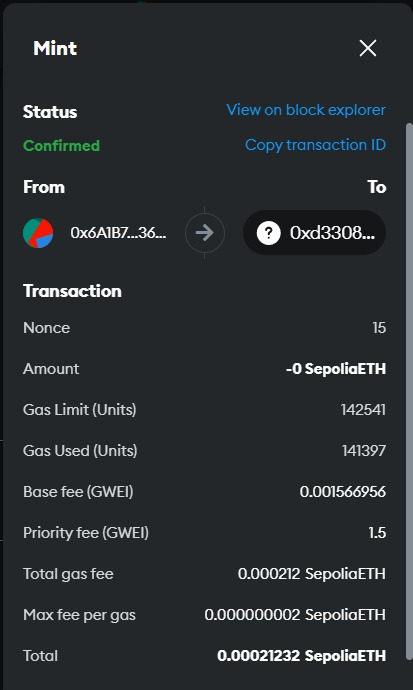
\includegraphics[scale=0.35]{gambar/riwayat_transaksi.jpeg}}
    % Keterangan gambar yang diinputkan
    \caption{Riwayat transaksi minting pada Metamask Wallet}
    % Label referensi dari gambar yang diinputkan
    \label{fig:minting}
    \end{figure}

    \item \emph{User} A akan melakukan \emph{minting} pada NFT dengan menggunakan MetaMask wallet, yang terhubung langsung ke Ethereum \emph{blockchain} melalui jaringan \emph{Sepolia Testnet}. Transaksi \emph{minting} ini mengkonfirmasi kreasi token baru di \emph{blockchain}, yang dicatat dengan detail transaksi seperti nonce, gas limit, dan biaya transaksi yang terdiri dari base fee dan priority fee. Proses ini mencatat NFT sebagai aset digital yang unik di \emph{blockchain}, memberikan hak kepemilikan digital kepada User A. Transaksi semacam ini memastikan keamanan dan transparansi dalam pencatatan kepemilikan aset digital, sekaligus mengintegrasikan NFT ke dalam ekosistem yang lebih luas di mana aset ini dapat diperdagangkan atau digunakan dalam aplikasi lain di masa depan.


    \item Tambahan dari gambar \ref*{fig:detail_transaksi_etherscan}, detail pada Etherscan memperlihatkan informasi kunci dari transaksi NFT yang dilakukan. \emph{Transaction hash} yang ditampilkan berfungsi sebagai pengenal unik transaksi, menunjukkan keberhasilannya pada \emph{blockchain}. Tanggal dan waktu transaksi juga tercatat, memberikan data penting mengenai kapan transaksi tersebut terjadi. Token yang terlibat adalah tipe ERC-721, standar untuk NFT yang memungkinkan representasi unik aset digital di Ethereum. Transaksi ini mencerminkan proses \emph{minting}, di mana NFT baru dibuat dan terdaftar di \emph{blockchain}, dan kemudian dialihkan dari alamat nol (menunjukkan penciptaan) ke alamat pemilik baru, yang dalam kasus ini adalah akun pertama yang melakukan \emph{minting}. Selain itu, biaya transaksi atau \emph{gas fee} yang relatif rendah menandakan efisiensi dalam pemrosesan transaksi tersebut di jaringan.

    \begin{figure} [H] \centering
    % Nama dari file gambar yang diinputkan
    \frame{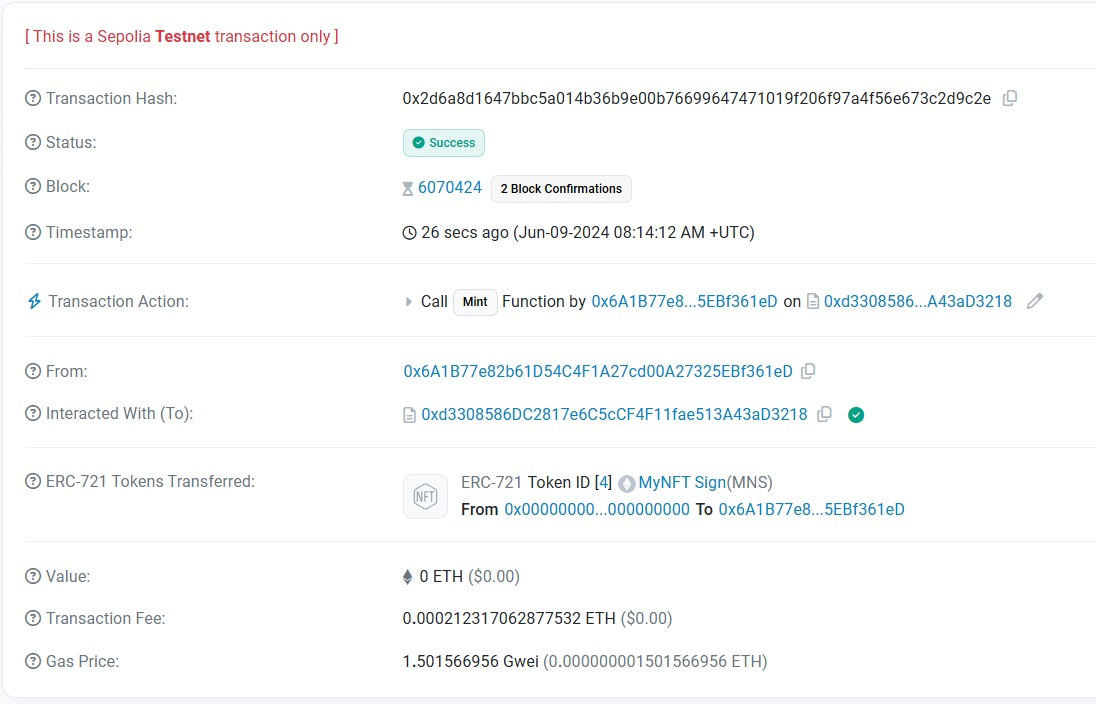
\includegraphics[scale=0.32]{gambar/detail_transaksi_etherscan.jpeg}}
    % Keterangan gambar yang diinputkan
    \caption{Detail transaksi pada Etherscan}
    % Label referensi dari gambar yang diinputkan
    \label{fig:detail_transaksi_etherscan}
    \end{figure}

    \item Pada gambar \ref*{fig:detail_nft_etherscan}, detail lebih lanjut mengenai NFT yang telah di-\emph{mint} juga dapat dilihat di Etherscan, seperti yang ditampilkan dalam gambar terlampir. Halaman Etherscan ini menyediakan data menyeluruh tentang NFT tersebut, termasuk alamat pemilik, alamat kontrak, dan pembuatnya. Setiap aspek dicatat dengan presisi untuk memastikan transparansi dan kemampuan dilacak dalam jaringan blockchain. Secara khusus, NFT ini, yang diidentifikasi sebagai "MyNFT Sign \#4", ditampilkan dengan ID token uniknya dan memastikan kepatuhan pada standar token ERC-721, yang menegaskan sifat non-fungible-nya. Tingkat detail ini penting untuk memverifikasi keaslian dan riwayat kepemilikan aset digital, membuat platform seperti Etherscan menjadi alat yang tak tergantikan dalam pengelolaan dan pertukaran NFT. Alat-alat ini juga meningkatkan keamanan transaksi digital dengan menyediakan jejak audit yang dapat diandalkan untuk setiap aset.

    \begin{figure} [H] \centering
    % Nama dari file gambar yang diinputkan
    \frame{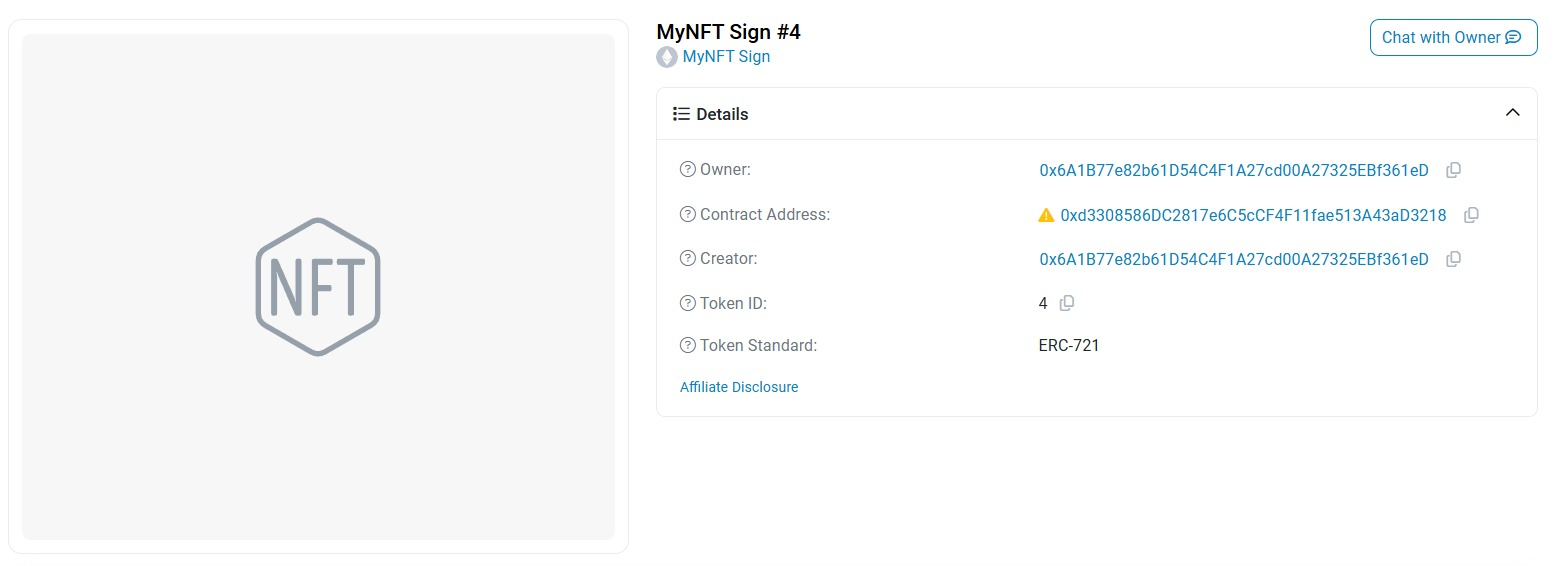
\includegraphics[scale=0.3]{gambar/detail_nft_etherscan.jpeg}}
    % Keterangan gambar yang diinputkan
    \caption{Detail NFT pada Etherscan}
    % Label referensi dari gambar yang diinputkan
    \label{fig:detail_nft_etherscan}
    \end{figure}
    
    \begin{figure} [H] \centering
    % Nama dari file gambar yang diinputkan
    \frame{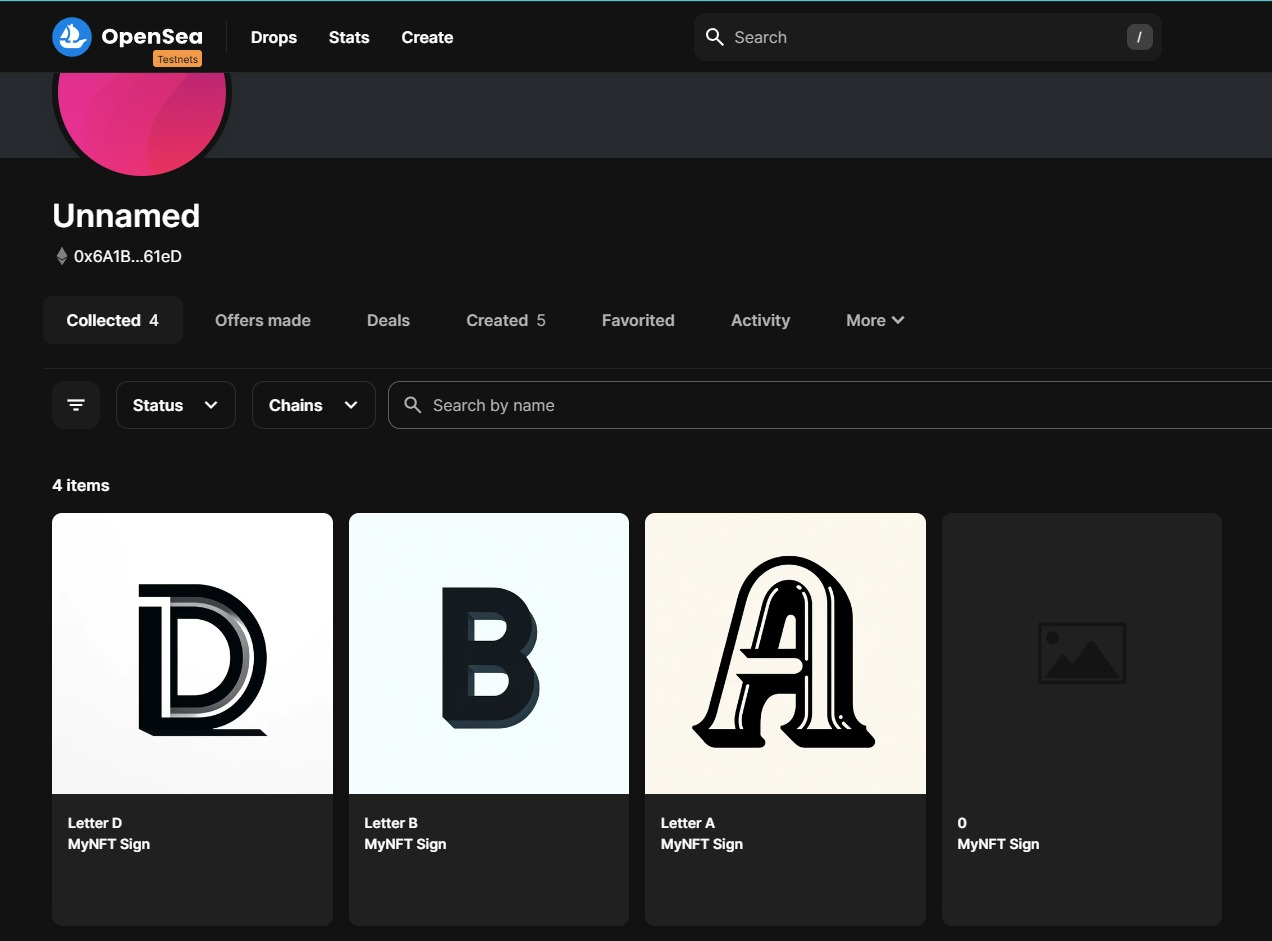
\includegraphics[scale=0.30]{gambar/nft_pada_opensea.jpeg}}
    % Keterangan gambar yang diinputkan
    \caption{NFT pada OpenSea}
    % Label referensi dari gambar yang diinputkan
    \label{fig:nft_opensea}
    \end{figure}

    \item Setelah proses \emph{minting} berhasil, seperti pada gambar \ref*{fig:nft_opensea} NFT yang telah di-\emph{minting} dapat dilihat pada platform OpenSea, yang merupakan pasar digital untuk aset kripto dan NFT. Dalam kasus pengujian ini, NFT yang telah di-minting adalah "Letter D", ditampilkan bersama dengan NFT lainnya yang telah dibuat oleh pengguna yang sama. Halaman OpenSea menampilkan berbagai detail seperti nama NFT, gambar, dan informasi lain yang relevan. Pengguna dapat melihat koleksi lengkap yang telah mereka mint atau beli. Setiap NFT ditampilkan dengan \emph{thumbnail} yang jelas, dan ketika di-klik, pengguna dapat melihat detail lebih lanjut seperti riwayat transaksi dan keaslian NFT tersebut. Ini memungkinkan pengguna untuk tidak hanya melihat koleksi mereka tetapi juga untuk berinteraksi dengan pasar, membuat penawaran, atau menjual NFT mereka.


    \item setelah NFT sudah terbuat, maka tahap berikutnya adalah melakukan \emph{lock} pada NFT yang akan dikirimkan ke \emph{user} B pada \emph{network} B'. Fungsi dari \emph{lock} ini untuk menjamin bahwa data token tidak diubah selama proses \emph{transfer}, menjaga kepercayaan dan keautentikan data NFT. Kemudian juga berguna untuk memberi sinyal kepada semua pihak terkait (pengguna, \emph{smart contract} di jaringan lain) bahwa token tersebut sedang dalam proses \emph{transfer}, dan operasi pada token harus ditangguhkan hingga proses selesai.

    \begin{figure} [H] \centering
    % Nama dari file gambar yang diinputkan
    \frame{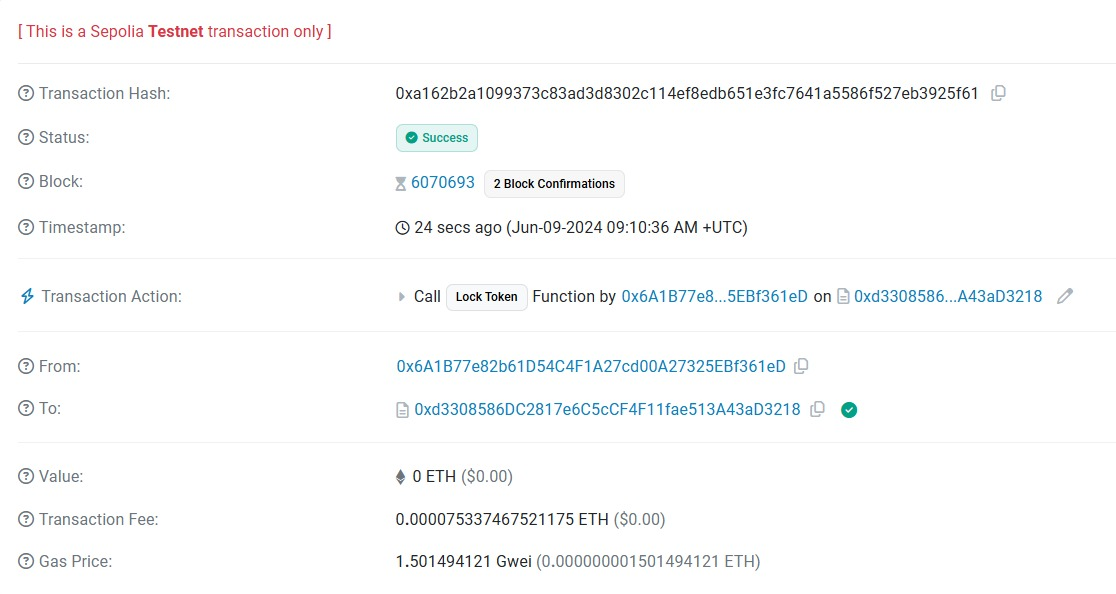
\includegraphics[scale=0.35]{gambar/lock_token.jpeg}}
    % Keterangan gambar yang diinputkan
    \caption{Detail fungsi \emph{Lock Token} pada Etherscan}
    % Label referensi dari gambar yang diinputkan
    \label{fig:locktoken}
    \end{figure}

    \item selesai melakukan proses \emph{lock token}, lalu fungsi \emph{bridge transfer} dapat dilaksanakan. Fungsi ini memfasilitasi transfer aman NFT antar \emph{blockchain} dengan memastikan bahwa NFT tersebut terkunci selama proses transfer dan memberikan visibilitas transparan tentang kejadian transfer melalui \emph{event} yang dicatat. Ini adalah komponen kunci dalam membangun aplikasi \emph{interoperable} yang memungkinkan aset \emph{digital} bergerak lintas ekosistem \emph{blockchain}.

    \begin{figure} [H] \centering
    % Nama dari file gambar yang diinputkan
    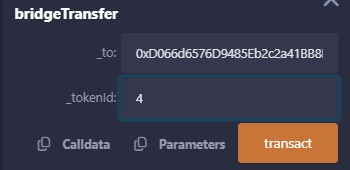
\includegraphics[scale=0.75]{gambar/bridge_transfer.jpeg}
    % Keterangan gambar yang diinputkan
    \caption{Parameter \emph{bridge transfer}}
    % Label referensi dari gambar yang diinputkan
    \label{fig:bridge_tranfer}
    \end{figure}

    \item pada gambar \ref{fig:bridge_tranfer} terdapat 2 parameter yaitu \texttt{"\emph{\_to}"}" yang digunakan untuk menerima parameter \emph{address} dari \emph{user} B dan juga parameter \texttt{"\emph{\_tokenId}"} untuk menerima argumen dari token NFT. Setelah dilakukan \emph{transact} maka akan dilanjutkan ke pembayaran pada Metamask Wallet.

    \begin{figure} [H] \centering
    % Nama dari file gambar yang diinputkan
    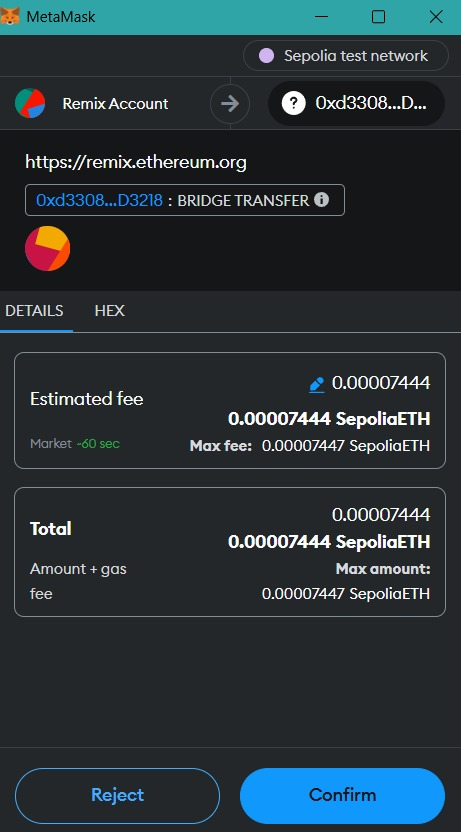
\includegraphics[scale=0.32]{gambar/verifikasi_metamask_wallet.jpeg}
    % Keterangan gambar yang diinputkan
    \caption{Pembayaran pada Metamask Wallet}
    % Label referensi dari gambar yang diinputkan
    \label{fig:metamask_pembayaran}
    \end{figure}

    \item setelah transaksi berhasil, \emph{record} dari transaksi tersimpan pada \emph{blockchain} yang dapat dilihat pada etherscan seperti pada gambar di bawah ini.

    \begin{figure} [H] \centering
    % Nama dari file gambar yang diinputkan
    \frame{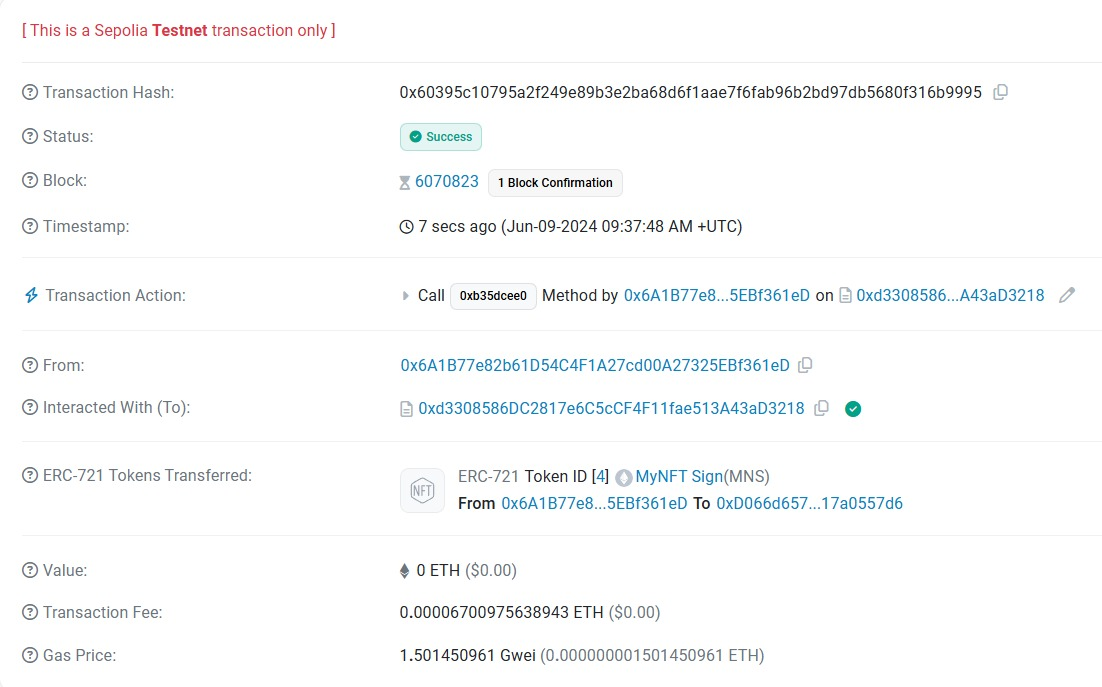
\includegraphics[scale=0.35]{gambar/detail_pada_etherscan.jpeg}}
    % Keterangan gambar yang diinputkan
    \caption{Detail pada Etherscan}
    % Label referensi dari gambar yang diinputkan
    \label{fig:detail_etherscan}
    \end{figure}

    \item pada etherscan juga terdapat detail pada NFT yang dapat dicek kepemilikannya. Jika dilihat dari gambar \ref{fig:detail_nft_etherscan} \emph{owner} dari NFT \#4 adalah \emph{address} dari \emph{user} A yang berada pada \emph{network Sepolia Ethereum Testnet}, lalu pada gambar di bawah ini setelah berhasil melakukan \emph{bridge transfer} kepemilikannya berganti kepada \emph{user} B yang berada pada \emph{network BNB Chain Testnet}.

    \begin{figure} [H] \centering
    % Nama dari file gambar yang diinputkan
    \frame{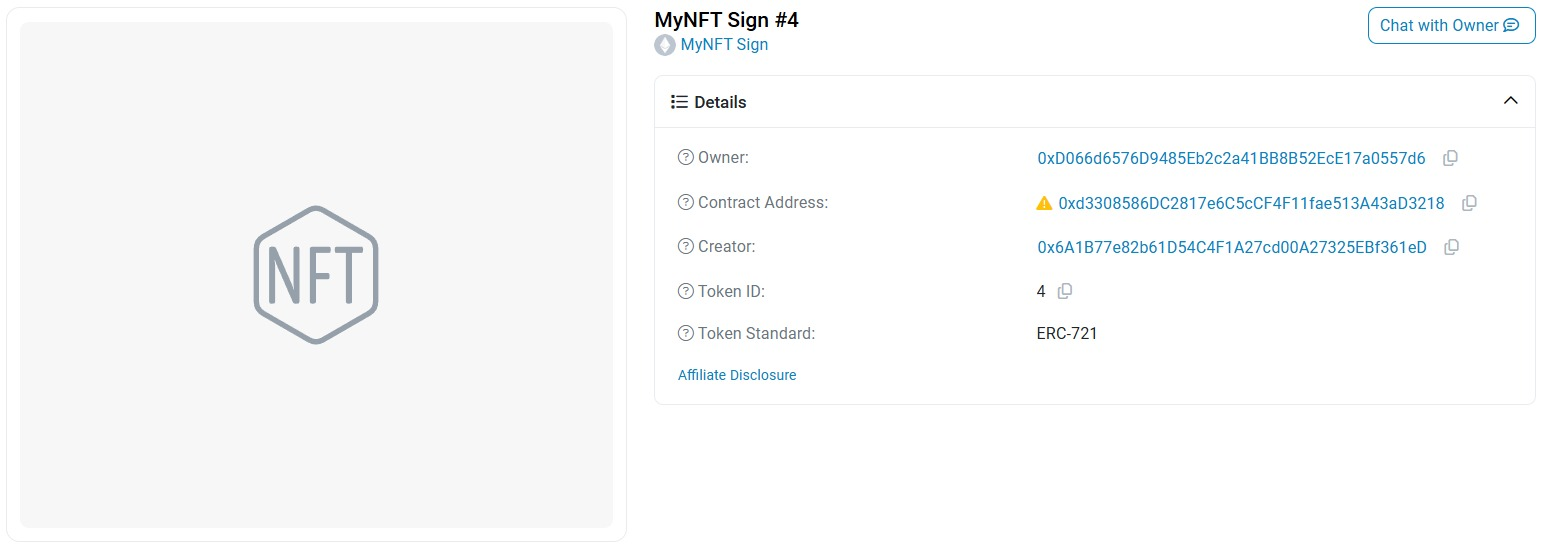
\includegraphics[scale=0.3]{gambar/nft_detail_etherscan2.jpeg}}
    % Keterangan gambar yang diinputkan
    \caption{Detail NFT pada Etherscan setelah \emph{bridge transfer}}
    % Label referensi dari gambar yang diinputkan
    \label{fig:nft_bridge_transfer}
    \end{figure}

    \item pada \emph{platform} OpenSea juga dapat dilihat pada akun milik \emph{adrress} \emph{user} B maka juga terdapat NFT yang telah terkirim ke alamatnya.

    \begin{figure} [H] \centering
    % Nama dari file gambar yang diinputkan
    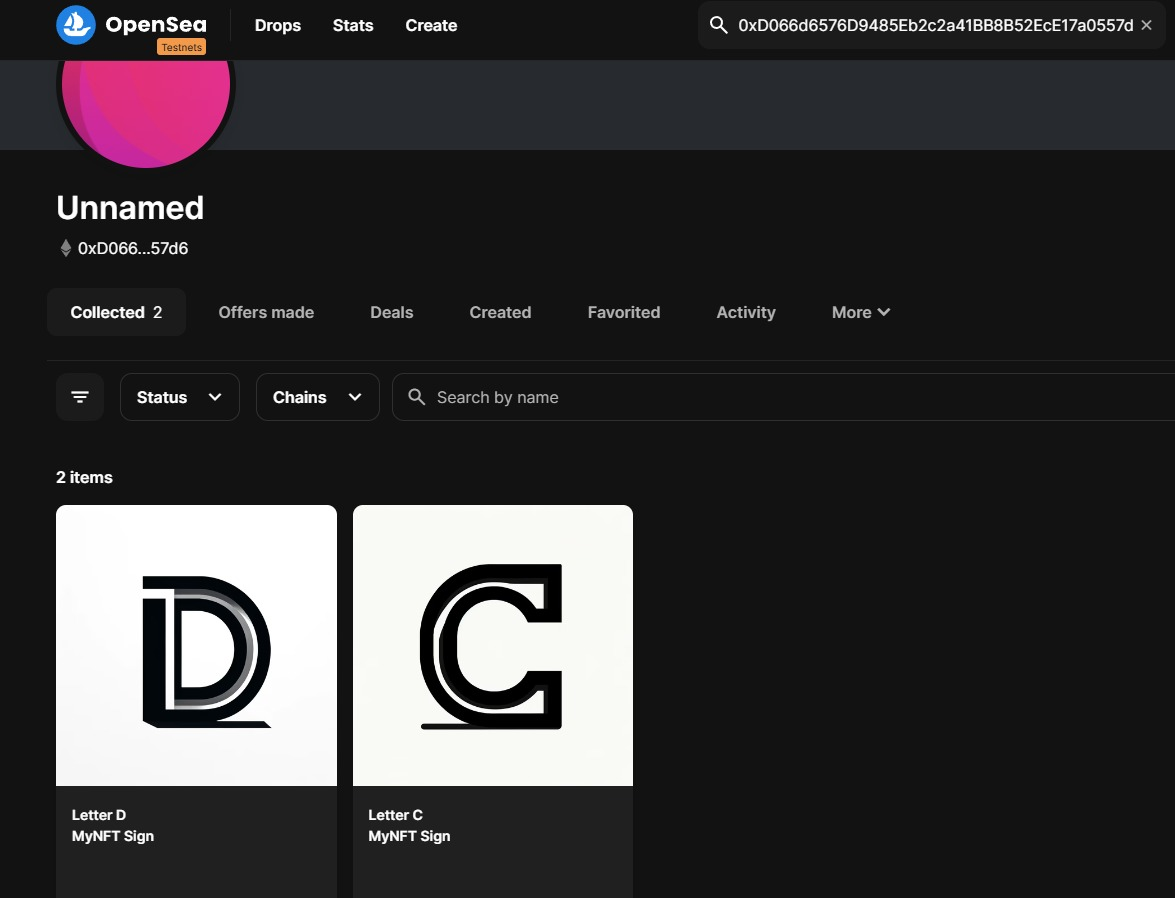
\includegraphics[scale=0.27]{gambar/nft_pada_opensea_2.jpeg}
    % Keterangan gambar yang diinputkan
    \caption{NFT pada OpenSea \emph{address} B}
    % Label referensi dari gambar yang diinputkan
    \label{fig:opensea2}
    \end{figure}
    
\end{itemize}

\subsection{Pengujian Integrasi \emph{Smart Contract} Dengan Web3.0}
Ekspektasi pengujian dari integrasi sistem \emph{smart contract} dengan web3.0 antara lain adalah sebagai berikut:
\begin{itemize}
    \item \emph{User} dapat melakukan integrasi akun Metamask Wallet dengan aplikasi web3.0

    \item \emph{User} dapat melakukan \emph{create listing} NFT untuk mengunggah NFT dari pemilik ke halaman \emph{Home} dan ke halaman \emph{My Listed Items}.

    \item \emph{User} dapat melakukan minting pada NFT yang telah dibuat dan kemudian terlihat pada halaman \emph{My Purchases}.

    \item \emph{User} yang memiliki NFT tersebut dapat melakukan \emph{transfer ownership} atau pindah kepemilikan dari alamat pengguna pemilik menuju ke alamat pengguna tujuan.

    \item \emph{User} yang memiliki NFT tersebut dapat melakukan fungsi seperti tahapan dalam melakukan \emph{bridge transfer} untuk melakukan pengiriman NFT dari alamat pengguna pada \emph{network} lokal ke alamat pengguna tujuan yang berada pada \emph{network} \emph{binance smart chain} ataupun \emph{sepolia ethereum}. 
\end{itemize}

Berikut merupakan langkah-langkah dari pengujian integrasi \emph{smart contract} dengan Web3.0 yang akan dilakukan:

\begin{itemize}
    \item \emph{User} akan mengakses web dengan menggunakan link yang dimunculkan secara lokal dengan melakukan run program lalu akan memunculkan link berupa \emph{localhost} yang dapat diakses pada platform seperti Google Chrome, Mozilla Firefox, atau Microsoft Edge, dan platform pengakses website lainnya.

    \begin{figure} [H] \centering
      % Nama dari file gambar yang diinputkan
      \frame{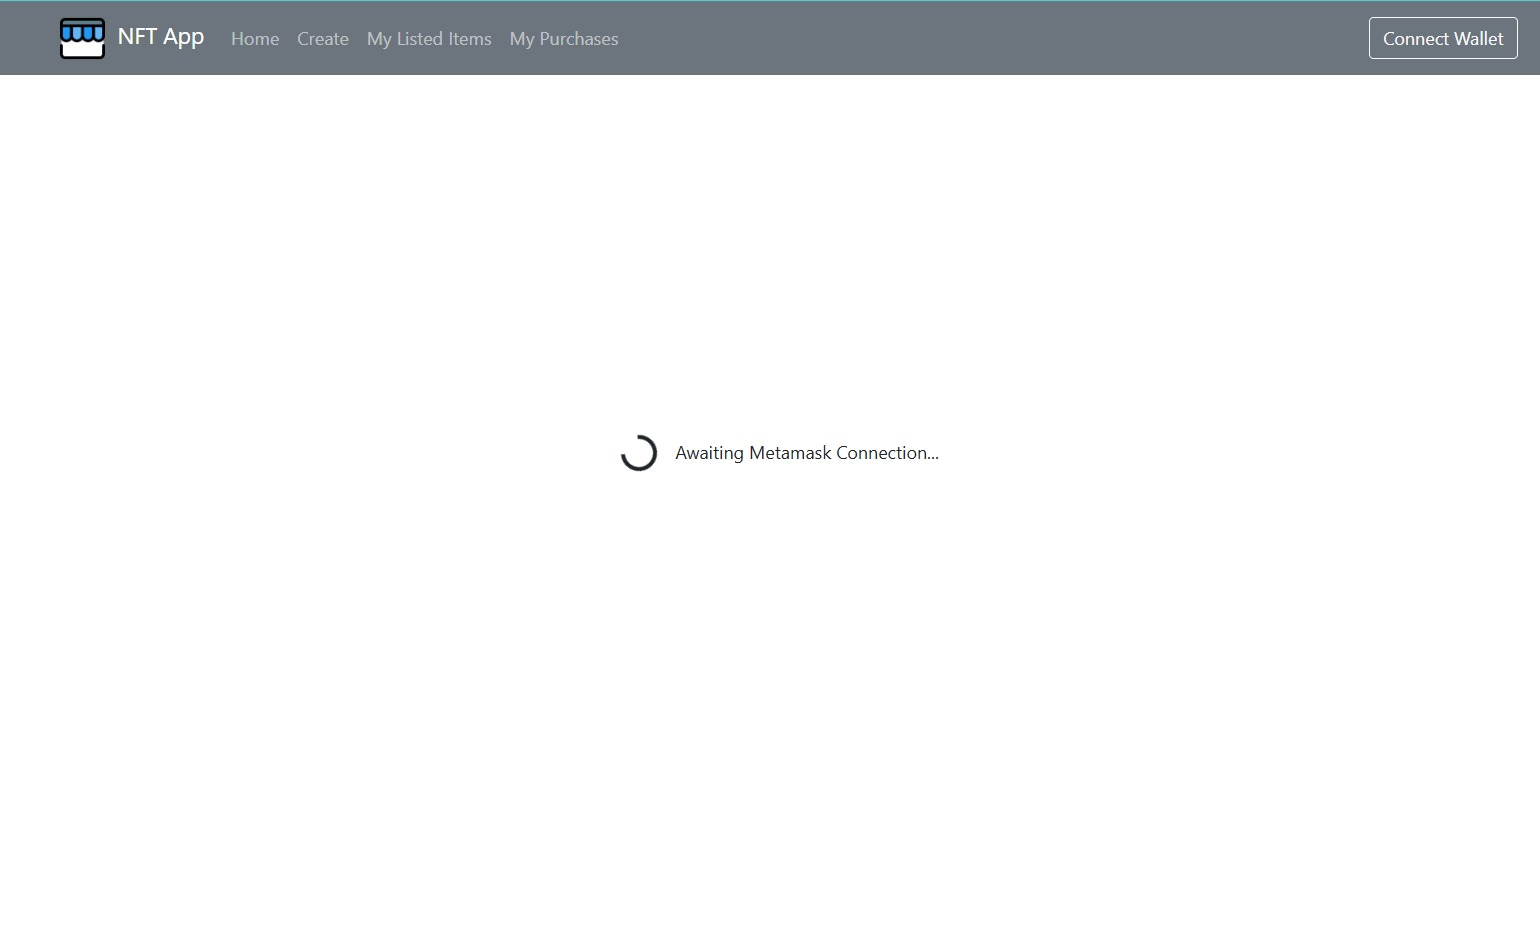
\includegraphics[scale=0.26]{gambar/login_page.jpg}}
      % Keterangan gambar yang diinputkan
      \caption{Tampilan awal dari web}
      % Label referensi dari gambar yang diinputkan
      \label{fig:web_interface}
      \end{figure}

    \item Pada gambar \ref{fig:web_interface} merupakan tampilan utama dari web, sebelum dapat melakukan \emph{load} data pengguna harus melakukan koneksi dengan akun Metamask Wallet. Integrasi harus dilakukan agar pengguna dapat mengakses tampilan lanjutan pada web. Integrasi tersebut dapat dilakukan dengan menekan tombol \emph{Connect Wallet} pada \emph{navigation bar} di pojok kanan atas.
    
    \begin{figure} [H] \centering
      \centering
      \begin{subfigure}{0.45\textwidth}
          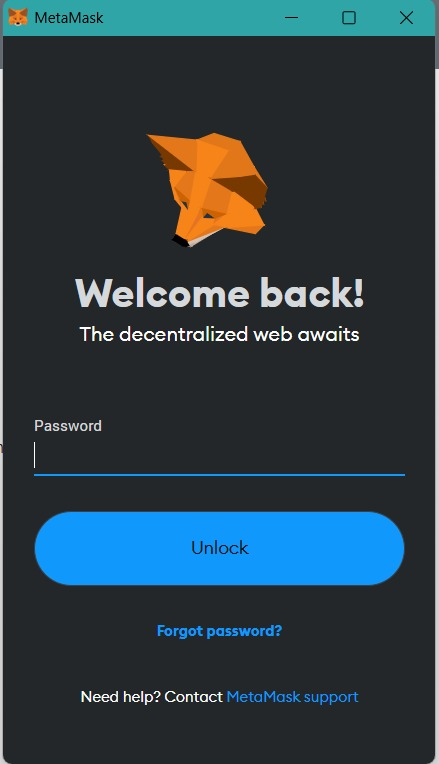
\includegraphics[scale=0.35]{gambar/integrasi_metamask.jpg}
          \caption{}
          \label{fig:intg_a}
      \end{subfigure}
      \hspace{5pt}
      \begin{subfigure}{0.45\textwidth}
        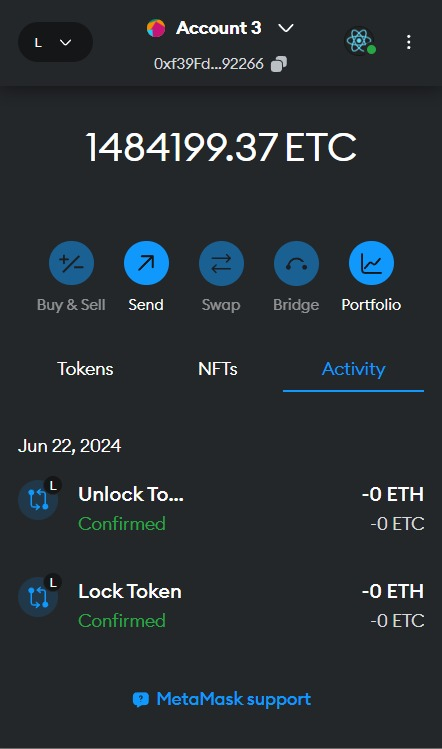
\includegraphics[scale=0.35]{gambar/metamask_konek.jpeg}
        \caption{}
        \label{fig:intg_b}
    \end{subfigure}
      \caption{Koneksi Metamask dengan Web}
      \label{fig:koneksi_web_metamask}
      \end{figure}

      \item Pada gambar \ref{fig:koneksi_web_metamask} adalah proses ketika melakukan integrasi dengan Metamask Wallet pada web. Ketika pengguna menekan tombol \emph{Connect Wallet} maka akan diarahkan kepada Metamask. Jika pengguna belum melakukan login pada Metamask maka pengguna akan disuruh login terlebih dahulu pada Metamask seperti pada gambar \ref{fig:intg_a}. Jika pengguna telah melakukan login ke akun Metamask, maka tampilannya akan seperti gambar \ref{fig:intg_b} yang di mana tampilan dari Metamask Wallet terdapat informasi \emph{address} dari akun dan juga \emph{balance} dari akun tersebut. Dikarenakan pada pengujian ini masih menggunakan \emph{localhost} maka \emph{balance} dari akun tersebut menggunakan milik Hardhat.
        
        \item Kemudian, kita akan menguji fungsionalitas sistem dengan fokus pada proses pengunggahan NFT, melakukan transaksi pembelian, serta mengirim NFT ke \emph{address} lain. Dalam skenario pengujian ini, seluruh aktivitas akan dilakukan dalam jaringan yang sama, yakni \emph{localhost}. Hal ini bertujuan untuk memastikan bahwa interaksi antar fungsi dalam \emph{smart contract} berjalan dengan lancar dan tanpa adanya gangguan eksternal yang mungkin terjadi dalam jaringan publik. Pengujian di \emph{localhost} memungkinkan kita untuk mengisolasi dan mengidentifikasi masalah fungsi dalam kondisi yang terkontrol sebelum memindahkannya ke jaringan tes yang lebih besar atau ke jaringan Ethereum utama. Selama proses ini, kita akan mengamati bagaimana sistem menangani proses-proses seperti penentuan kepemilikan, transaksi pembayaran, dan transfer kepemilikan antar pengguna, yang semuanya merupakan komponen penting dari aplikasi berbasis NFT. Pengujian ini juga mencakup verifikasi keamanan dan integritas data untuk memastikan bahwa tidak ada celah yang dapat dimanfaatkan oleh pengguna jahat dalam ekosistem.
      
      \begin{figure} [H] \centering
        % Nama dari file gambar yang diinputkan
        \frame{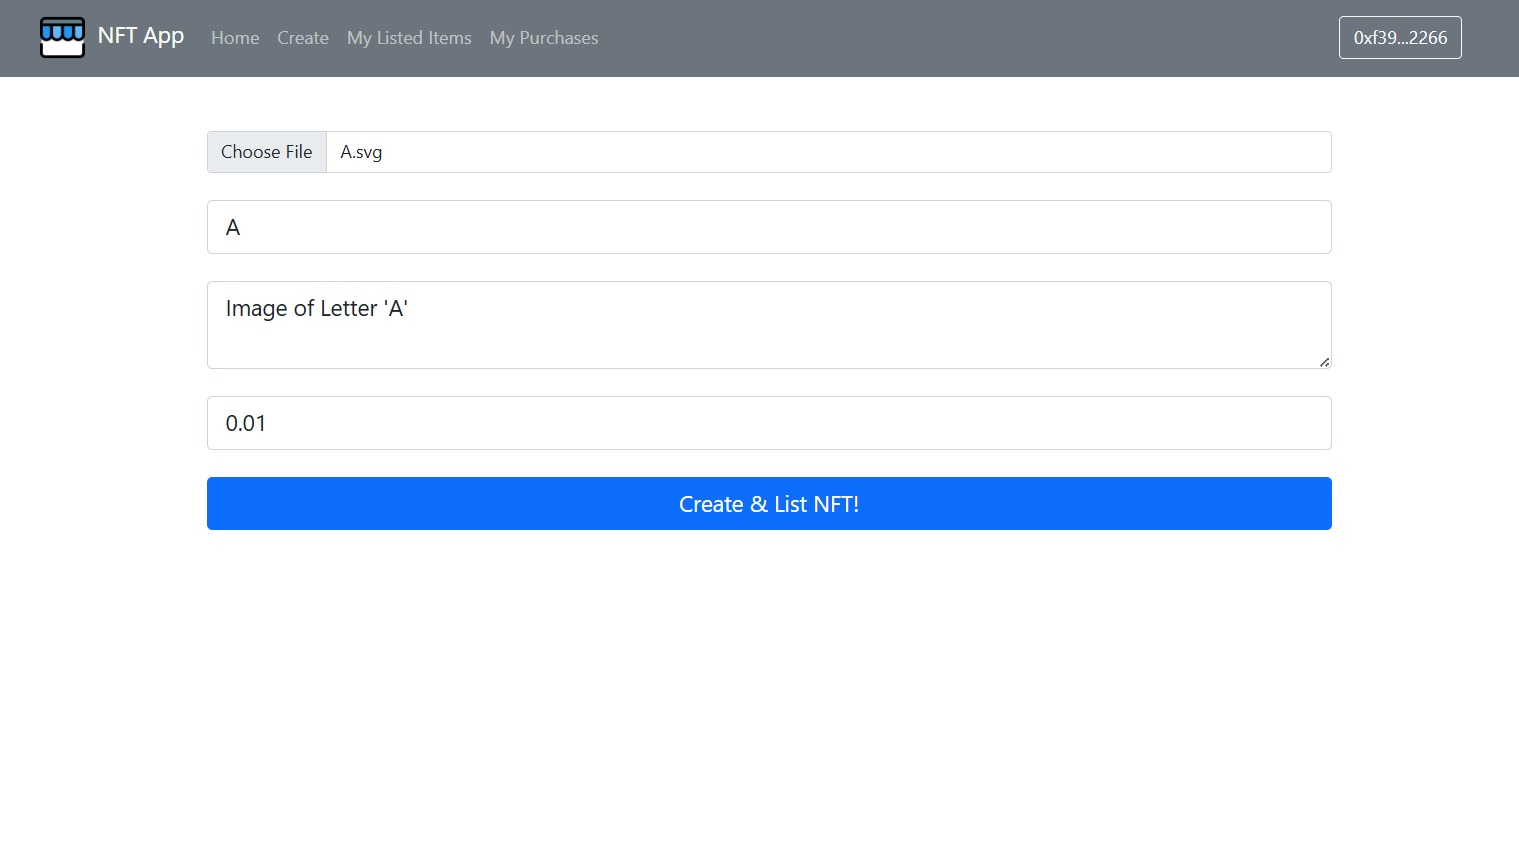
\includegraphics[scale=0.27]{gambar/create_nft.jpg}}
        % Keterangan gambar yang diinputkan
        \caption{Melakukan pengunggahan NFT pada halaman \emph{create}}
        % Label referensi dari gambar yang diinputkan
        \label{fig:createnft}
        \end{figure}

      \item Pada tahap awal ini pengguna melakukan pengunggahan NFT pada halaman \emph{create}. Pengguna memasukkan detail-detail dari NFT yang ingin diunggah seperti gambar, nama, deskripsi, dan juga harga dalam mata uang \emph{ethereum}. Pada pengujian ini pengguna memasukkan NFT gambar "A" seperti pada pengujian \emph{smart contract} sebelumnya. Setelah pengguna menekan tombol "\emph{Create \& List NFT!}" maka akan muncul \emph{pop up window} dari Metamask Wallet yang digunakan untuk membayar \emph{gas} atau fee dari melakukan eksekusi kode \emph{smart contract}. 
      
       \begin{figure} [H] \centering
      \centering
      \begin{subfigure}{0.45\textwidth}
          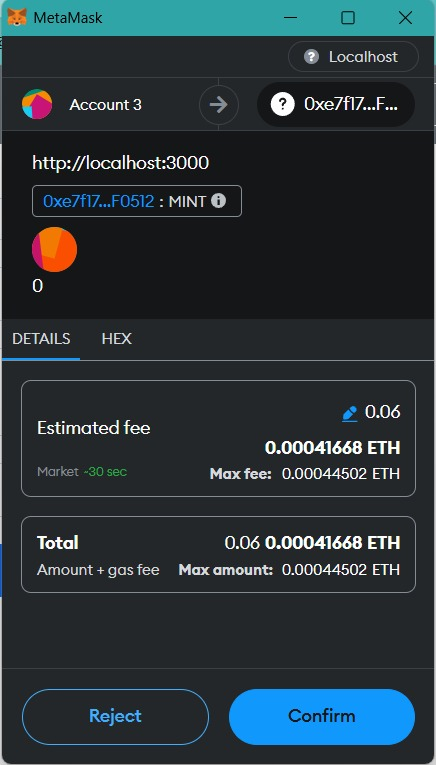
\includegraphics[scale=0.32]{gambar/confirm_create.jpg}
          \caption{}
          \label{fig:payipfs-a}
      \end{subfigure}
      \hspace{5pt}
      \begin{subfigure}{0.45\textwidth}
        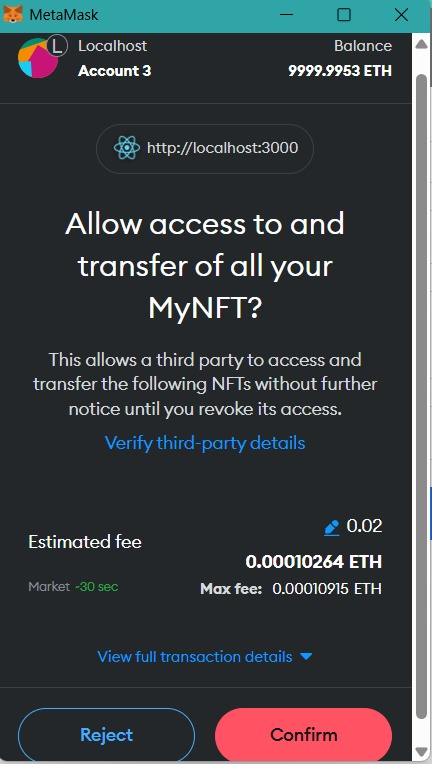
\includegraphics[scale=0.32]{gambar/confirm_upload.jpg}
        \caption{}
        \label{fig:payipfs-b}
    \end{subfigure}
      \caption{Pembayaran gas IPFS menggunakan Metamask Wallet}
      \label{fig:koneksi_web_metamask}
      \end{figure}
      
        \item Gambar \ref{fig:payipfs-a} adalah pembayaran \emph{gas} dari metamask wallet. Pembayaran \emph{gas} tersebut terjadi karena pada \emph{smart contract} terjadi proses pengunggahan gambar NFT ke platform penyedia IPFS. Pada web ini kita mengintegrasikan dengan platform bernama Pinata. Pinata sendiri merupakan platform penyedia servis IPFS. Kemudian juga terdapat konfirmasi pada gambar \ref{fig:payipfs-b}, konfirmasi ini dilakukan karena melakukan integrasi dengan platform Pinata yang kita gunakan sebagai penyedia servis IPFS. 
        
        \item Setelah berhasil melakukan konfirmasi pembayaran gas melalui MetaMask, NFT yang telah dibuat melalui halaman "Create" pada aplikasi akan diunggah ke platform Pinata. Platform Pinata ini berfungsi sebagai penyedia layanan penyimpanan dan pengelolaan file berbasis teknologi blockchain, yang menggunakan sistem InterPlanetary File System (IPFS) untuk memastikan keamanan dan ketahanan data.
        
        \begin{figure} [H] \centering
          % Nama dari file gambar yang diinputkan
          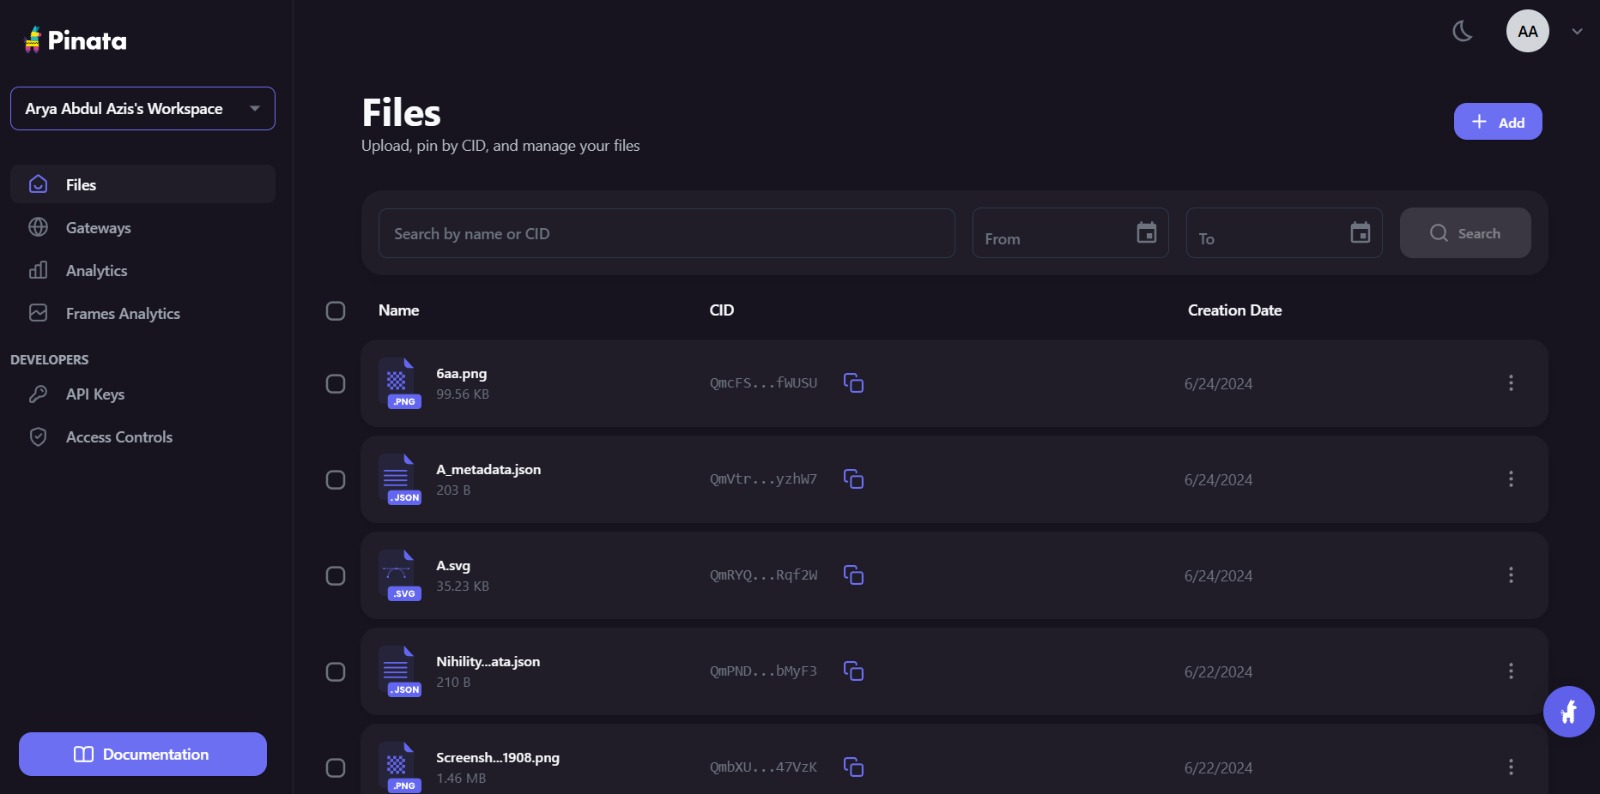
\includegraphics[scale=0.25]{gambar/pinata.jpeg}
          % Keterangan gambar yang diinputkan
          \caption{Data dari NFT ter-\emph{upload} pada platform Pinata}
          % Label referensi dari gambar yang diinputkan
          \label{fig:pinata}
          \end{figure}

        \item Dalam platform Pinata seperti pada gambar \ref{fig:pinata}, setiap file yang diunggah, termasuk gambar untuk NFT, akan diberikan Content Identifier (CID) unik yang memudahkan pelacakan dan akses tanpa perlu mengkhawatirkan perubahan isi file, karena CID ini akan berubah jika konten file berubah. Hal ini sangat penting dalam ekosistem NFT di mana keaslian dan keunikan konten harus terjamin. Di Pinata, pengguna dapat dengan mudah melihat semua file yang telah diunggah, mengatur akses, dan memantau penggunaan dan analisis lalu lintas file. Fitur ini memungkinkan pembuat konten NFT untuk tidak hanya menyimpan aset digital mereka dengan aman tetapi juga mengelola distribusi mereka dengan lebih efektif dalam pasar digital. Keseluruhan proses ini mengintegrasikan teknologi blockchain dengan aplikasi web, memastikan bahwa setiap pembelian dan transfer NFT dapat dilacak dan diverifikasi secara transparan dan aman. Pinata tidak hanya menyediakan solusi penyimpanan yang efisien dan aman tetapi juga menawarkan antarmuka yang ramah pengguna, memudahkan para pengguna, terutama para pembuat NFT, untuk mengunggah dan mengelola aset digital mereka dengan mudah. Fitur pencarian dan pengelolaan file yang intuitif memungkinkan pengguna untuk mengakses dan mengatur koleksi NFT mereka tanpa hambatan, memastikan bahwa aset digital dapat dikelola dan diakses dengan cepat sesuai kebutuhan. Lebih lanjut, Pinata mendukung integrasi dengan berbagai platform dan marketplace NFT, sehingga memperluas jangkauan dan visibilitas aset digital yang disimpan di dalamnya. Hal ini memberikan nilai tambah bagi para pembuat dan kolektor NFT dalam mendistribusikan dan memperdagangkan karya mereka di berbagai platform dengan mudah dan aman. Melalui Pinata, pembuat NFT dapat memastikan bahwa setiap aset digital tidak hanya aman tetapi juga siap untuk diintegrasikan dan digunakan dalam ekosistem blockchain yang lebih luas.
      
        \begin{figure} [H] \centering
          % Nama dari file gambar yang diinputkan
          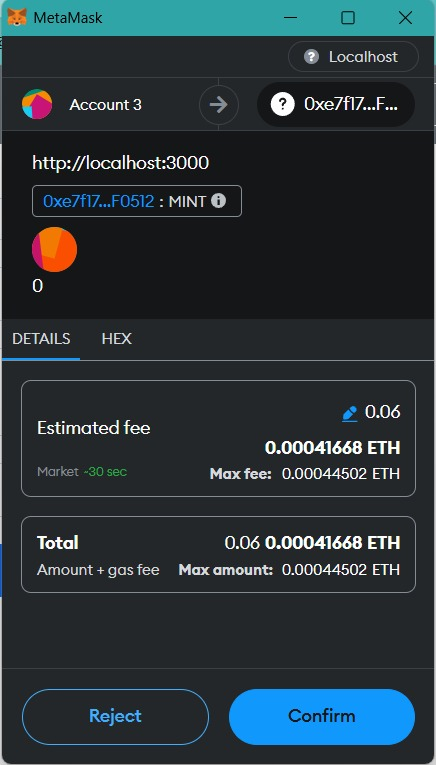
\includegraphics[scale=0.43]{gambar/confirm_create.jpg}
          % Keterangan gambar yang diinputkan
          \caption{Melakukan konfirmasi \emph{minting} NFT pada Metamask Wallet}
          % Label referensi dari gambar yang diinputkan
          \label{fig:makenft}
          \end{figure}
      
      \item 
      Pada gambar \ref{fig:makenft}, ditampilkan jendela konfirmasi MetaMask yang digunakan untuk memberikan persetujuan atas transaksi minting NFT. Dalam jendela ini, pengguna diminta untuk mengkonfirmasi atau menolak transaksi yang sedang diinisiasi dari aplikasi yang dihosting pada localhost:3000. Proses ini memastikan bahwa pengguna memahami dan menyetujui semua detail transaksi sebelum melanjutkan. Di dalam jendela konfirmasi, jumlah ETH yang akan ditransfer adalah 0, yang menandakan bahwa transaksi ini mungkin hanya melibatkan biaya gas, tanpa ada transfer dana tambahan yang terlibat. "Estimated fee" atau perkiraan biaya gas untuk transaksi ini ditampilkan, dengan jumlah minimal yang ditetapkan serta maksimum yang mungkin diperlukan, memberikan transparansi tentang biaya yang dapat dikeluarkan untuk memproses transaksi ini. Selain itu, MetaMask juga menyediakan informasi mengenai durasi estimasi untuk penyelesaian transaksi di pasar yang ditandai dengan "+30 sec", yang berarti transaksi diharapkan terjadi dalam waktu sekitar 30 detik.

      
      \begin{figure} [H] \centering
        % Nama dari file gambar yang diinputkan
        \frame{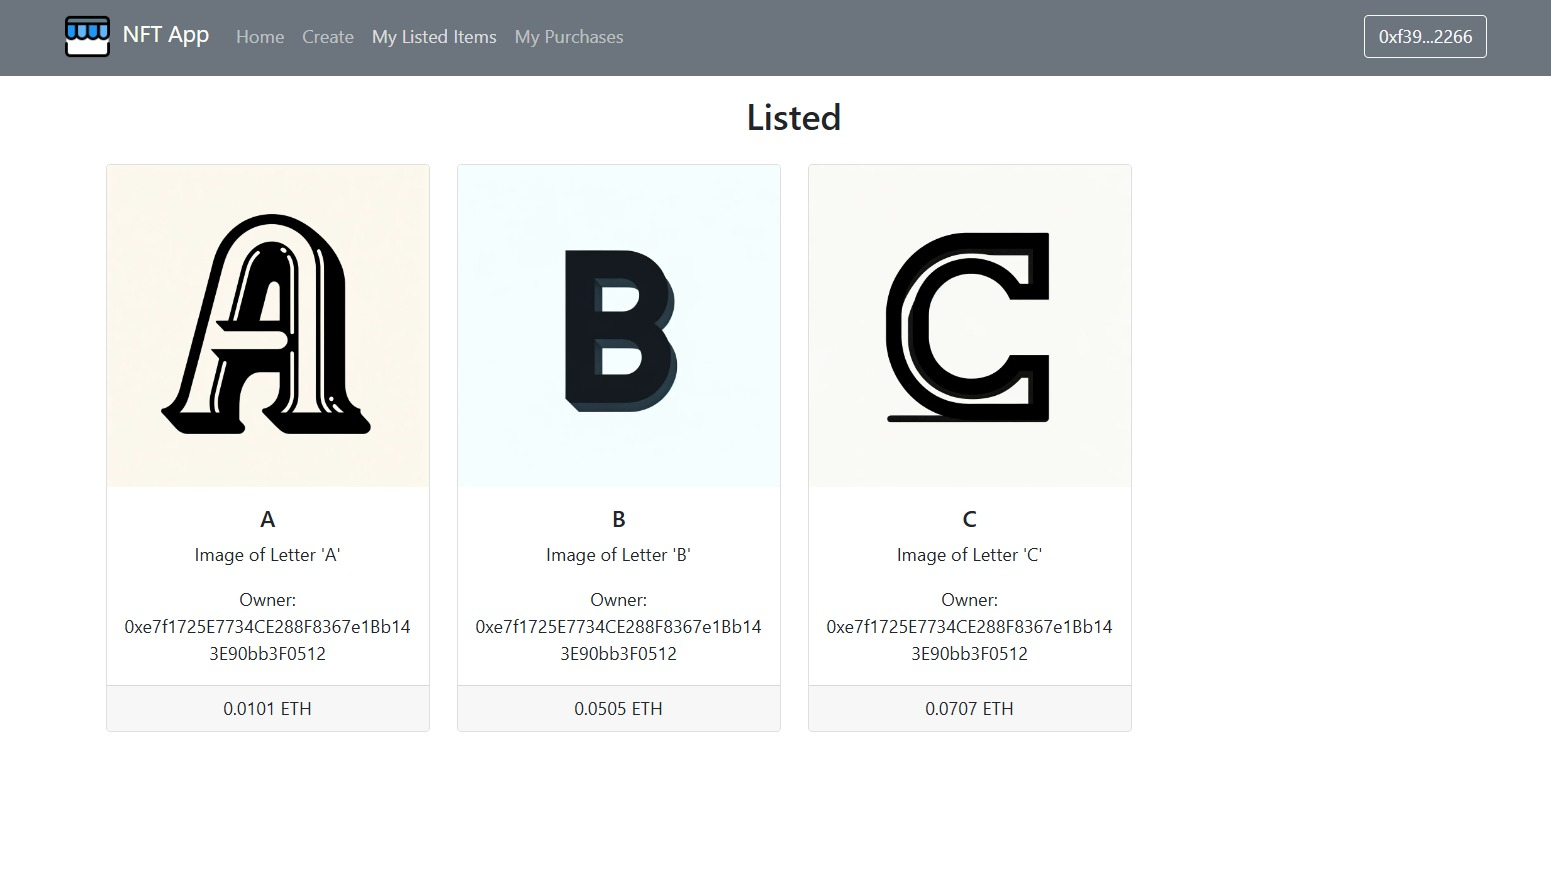
\includegraphics[scale=0.26]{gambar/listed_nft.jpeg}}
        % Keterangan gambar yang diinputkan
        \caption{NFT yang telah di-\emph{minting} terlihat pada halaman \emph{My listed items}}
        % Label referensi dari gambar yang diinputkan
        \label{fig:listeditem}
      \end{figure}

      \item Setelah pengguna menyelesaikan proses minting NFT dan melakukan konfirmasi melalui MetaMask seperti yang dijelaskan sebelumnya, NFT yang baru dibuat akan muncul pada halaman "My Listed Items" dalam aplikasi. Halaman ini berfungsi sebagai galeri pribadi pengguna dimana semua NFT yang telah mereka buat dan daftarkan untuk dijual ditampilkan. Dalam contoh yang ditampilkan pada gambar, NFT dengan desain huruf "A" yang telah berhasil di-\emph{list} tampak dengan harga yang tertera di bawah gambar yaitu 0.0101 ETH. Kemudian juga terdapat NFT dengan desain huruf "B" yang berhasil di-\emph{list} dengan harga yang tertera di gambar yaitu 0.0505 ETH, dan juga NFT dengan desain huruf "C" yang berhasil di-\emph{list} dengan harga yang tertera di gambar yaitu 0.0707 ETH. Hal ini menandakan bahwa NFT ini siap untuk dibeli oleh pengguna lain. Setiap NFT yang terdaftar di halaman ini akan menampilkan gambar yang berkaitan dengan NFT tersebut, yang merupakan hasil unggahan pengguna ke IPFS, dan metadata lainnya seperti nama dan deskripsi juga akan ditampilkan jika pengguna telah menyertakannya saat proses minting.
      
      \item Setelah menyelesaikan proses pengunggahan dan minting NFT, NFT yang baru dibuat juga dapat dilihat di halaman utama (\emph{home page}) web aplikasi NFT. Gambar yang disajikan menunjukkan NFT berupa gambar huruf "A", yang ditampilkan dengan label dan harga penjualan. Di halaman utama ini, NFT tidak hanya dipamerkan tetapi juga siap untuk dibeli oleh pengguna lain. Dalam tampilan ini, setiap NFT yang di-list akan dilengkapi dengan tombol "\emph{Buy}" yang memungkinkan pengguna langsung membeli NFT tersebut. Tombol ini memfasilitasi pembelian langsung tanpa perlu navigasi ke halaman lain, memberikan kemudahan bagi pembeli untuk segera mengakuisisi aset digital yang diinginkan. 

      \begin{figure} [H] \centering
        % Nama dari file gambar yang diinputkan
        \frame{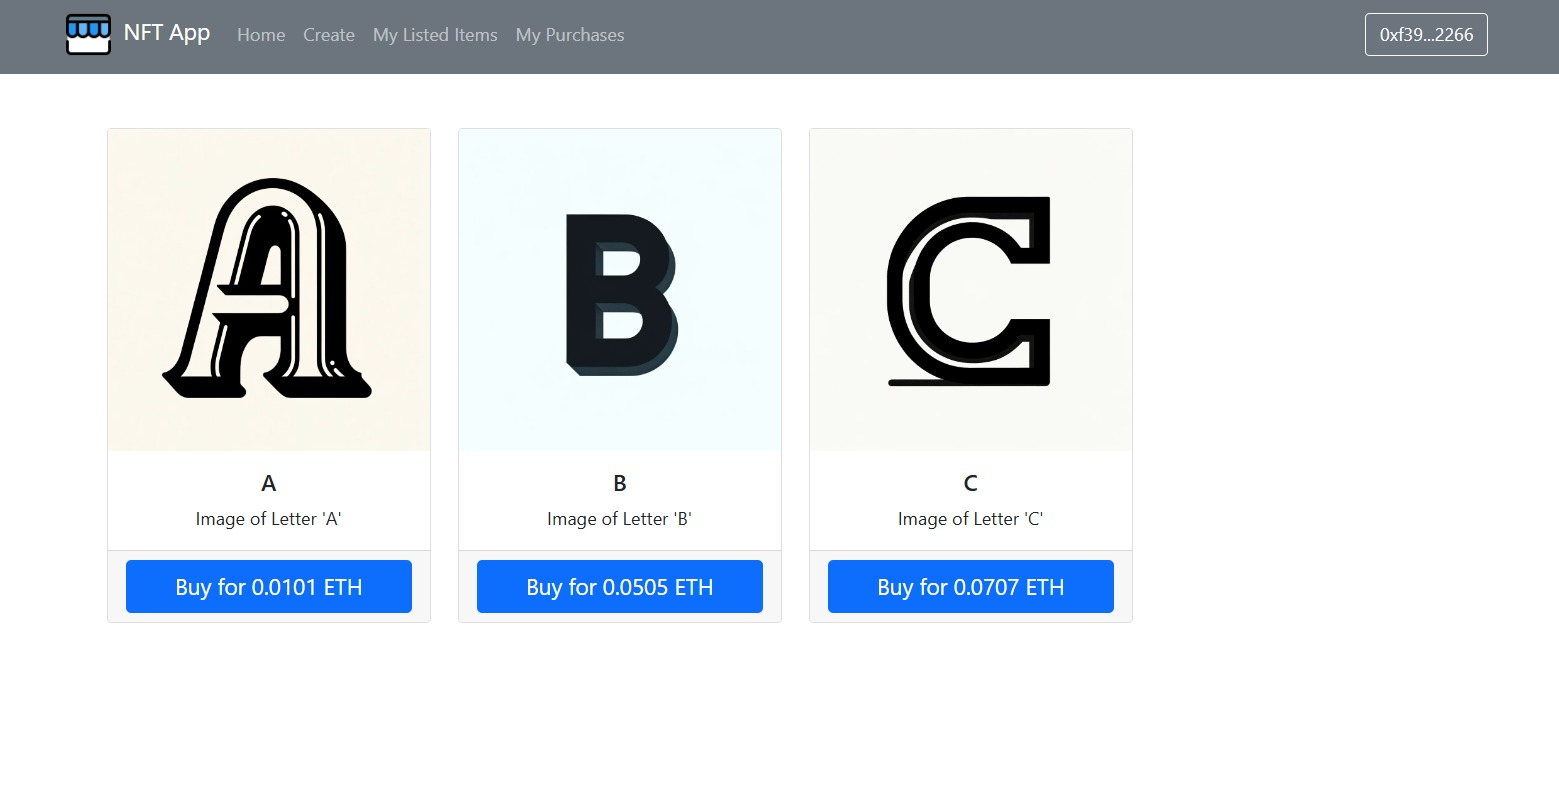
\includegraphics[scale=0.26]{gambar/nft_listed_home.jpeg}}
        % Keterangan gambar yang diinputkan
        \caption{NFT yang telah di-\emph{minting} terlihat pada halaman \emph{home}}
        % Label referensi dari gambar yang diinputkan
        \label{fig:listhome}
        \end{figure}

        \item Pada gambar \ref{fig:listhome} ketika tombol tersebut diklik, transaksi akan diproses melalui MetaMask atau wallet digital lainnya yang telah disinkronkan dengan aplikasi. Halaman ini dirancang untuk memberikan pengalaman pengguna yang intuitif dan efisien, di mana pembeli dapat dengan cepat mengakses NFT yang mereka inginkan dan melihat informasi penting seperti nama, deskripsi, dan harga NFT. Ini tidak hanya memperkuat transparansi dan aksesibilitas dalam pasar NFT tetapi juga mendorong interaksi langsung dan spontan antara pembeli dan aset digital.

      \item Sebelum melakukan pembelian NFT, pengguna harus mengganti akun yang aktif pada Metamask Wallet ke "Account 4", yang telah disiapkan khusus sebagai akun kedua. Akun ini berfungsi sebagai platform untuk melakukan transaksi pembelian, memungkinkan pengguna untuk menguji proses pembelian NFT yang telah diunggah oleh akun pertama. Penggunaan akun kedua ini sangat penting dalam pengujian fungsionalitas transfer kepemilikan, memastikan bahwa seluruh proses berjalan lancar dan tanpa hambatan. 
      
      \begin{figure} [H] \centering
        % Nama dari file gambar yang diinputkan
        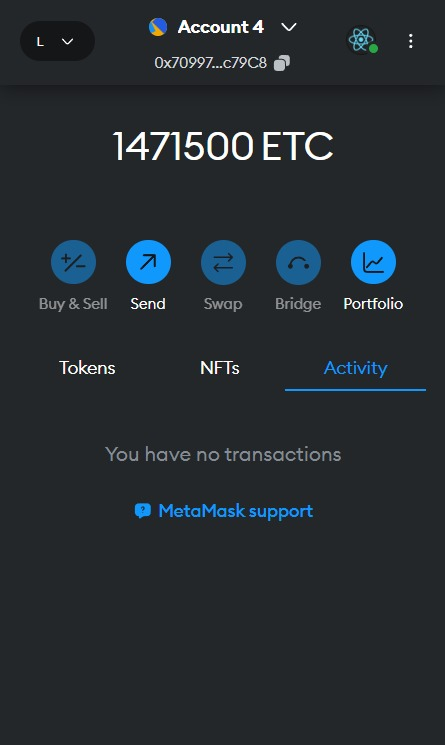
\includegraphics[scale=0.47]{gambar/metamask_akun_2.jpeg}
        % Keterangan gambar yang diinputkan
        \caption{Akun Metamask kedua}
        % Label referensi dari gambar yang diinputkan
        \label{fig:akun2}
        \end{figure}

        \item Pada gambar \ref{fig:makeitem} ketika pengguna memilih untuk membeli sebuah NFT yang ditampilkan pada halaman utama aplikasi, mereka akan mengklik tombol "Buy" yang berada di bawah item yang diinginkan. Langkah ini memicu proses transaksi, di mana Metamask Wallet secara otomatis terbuka, meminta pengguna untuk mengonfirmasi pembelian. Layar Metamask yang muncul merupakan jendela penting yang menampilkan detail transaksi yang harus diperiksa pengguna sebelum mereka melanjutkan. Dalam jendela konfirmasi ini, pengguna akan melihat jumlah total Ethereum (ETH) yang harus dibayarkan, yang sudah termasuk estimasi biaya gas. Biaya gas ini adalah biaya yang dibutuhkan untuk memproses transaksi di jaringan Ethereum, dan nilainya dapat berfluktuasi berdasarkan kepadatan trafik jaringan saat itu. Metamask memberikan dua estimasi: "Estimated fee" yang merupakan perkiraan biaya gas yang akan dikenakan, dan "Max fee" yang menunjukkan batas maksimal biaya yang mungkin ditarik jika kondisi jaringan berubah secara signifikan selama transaksi diproses. Proses ini tidak hanya memindahkan kepemilikan NFT dari penjual ke pembeli, tetapi juga memperbarui semua record yang berkaitan di \emph{blockchain}. Setelah konfirmasi berhasil, NFT akan muncul dalam koleksi pengguna di aplikasi, dan item tersebut akan dihapus dari daftar yang tersedia untuk dijual, menandakan bahwa transaksi telah selesai secara resmi dan NFT kini memiliki pemilik baru. Proses ini menunjukkan integrasi yang mulus antara platform NFT berbasis web dengan teknologi wallet \emph{blockchain} seperti Metamask, menawarkan pengalaman pengguna yang aman dan efisien.
    
      \begin{figure} [H] \centering
        % Nama dari file gambar yang diinputkan
        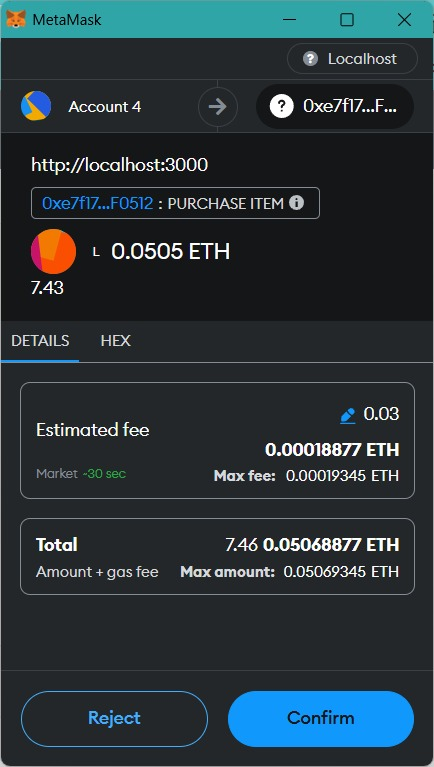
\includegraphics[scale=0.45]{gambar/make_item.jpeg}
        % Keterangan gambar yang diinputkan
        \caption{Proses pembelian NFT}
        % Label referensi dari gambar yang diinputkan
        \label{fig:makeitem}
        \end{figure}
      

    \begin{figure} [H] \centering
    % Nama dari file gambar yang diinputkan
    \frame{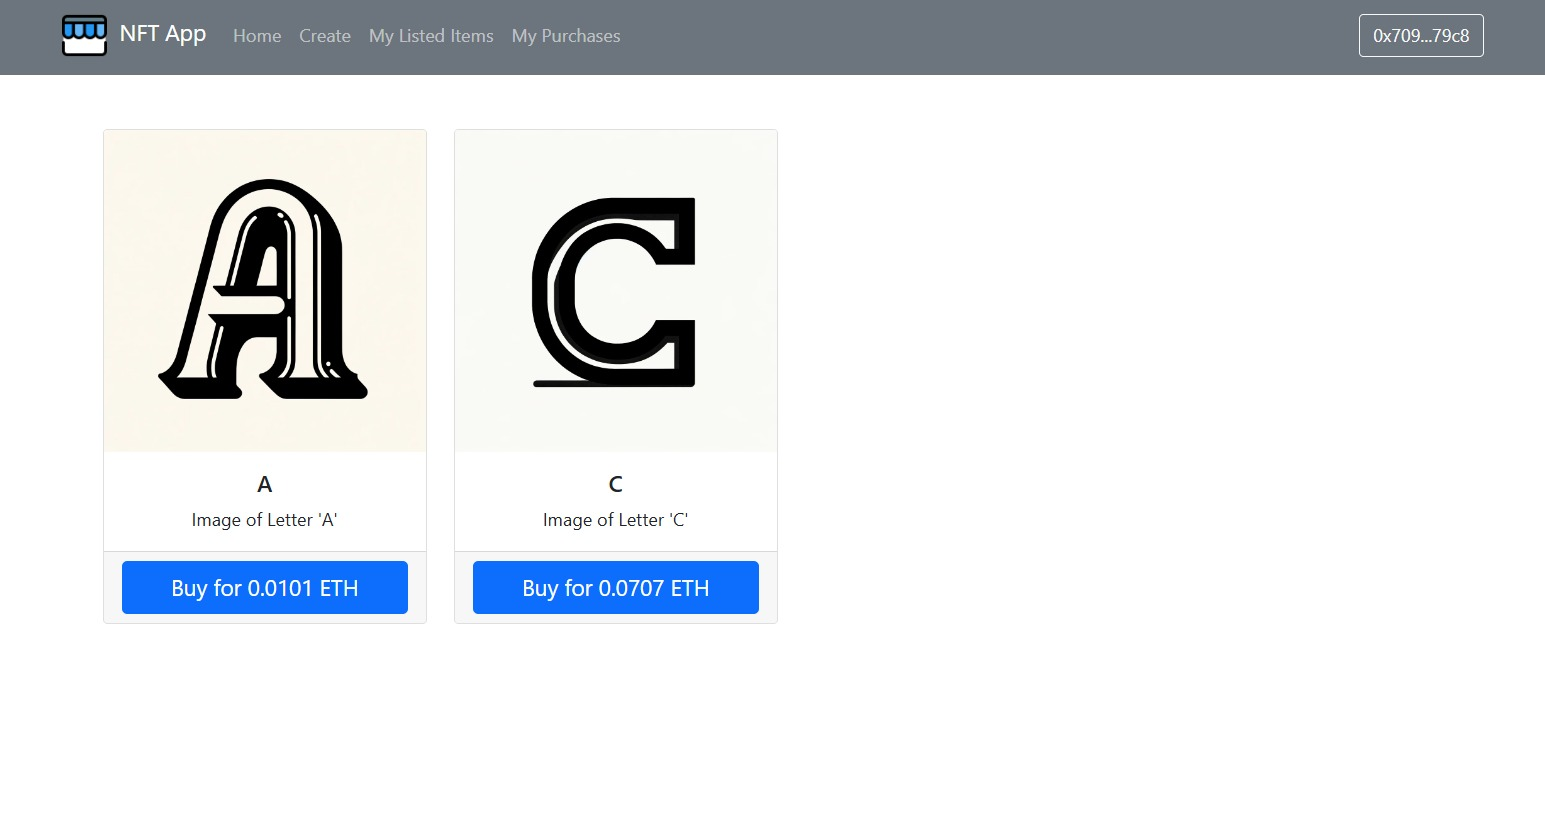
\includegraphics[scale=0.25]{gambar/home_setelah_nft_dibeli.jpg}}
    % Keterangan gambar yang diinputkan
    \caption{Tampilan \emph{home} setelah NFT dibeli}
    % Label referensi dari gambar yang diinputkan
    \label{fig:home_setelah_dibeli}
    \end{figure}
    
    \item Pada gambar \ref{fig:home_setelah_dibeli}, NFT B telah berhasil dibeli oleh \emph{user} B. Proses pembelian ini menyebabkan perubahan langsung pada tampilan halaman \emph{home}, di mana sistem secara otomatis melakukan pembaruan atau \emph{refresh}. Sebelum transaksi, seperti yang terlihat pada gambar \ref{fig:listhome}, ada tiga NFT yang tersedia untuk dibeli. Namun, setelah NFT B dibeli, jumlah NFT yang ditampilkan berkurang menjadi dua. Hal ini menunjukkan bahwa sistem berhasil memperbarui daftar NFT yang tersedia sesuai dengan status penjualan terkini. Proses otomatis ini memastikan bahwa informasi yang disajikan kepada pengguna selalu akurat dan terkini, mencerminkan perubahan real-time pada inventori NFT yang ada dalam platform. Perubahan ini tidak hanya memudahkan pengguna dalam melihat NFT yang masih tersedia tetapi juga meningkatkan pengalaman pengguna dengan menampilkan data yang akurat dan responsif terhadap interaksi pengguna di platform.
    
      \begin{figure} [H] \centering
        % Nama dari file gambar yang diinputkan
        \frame{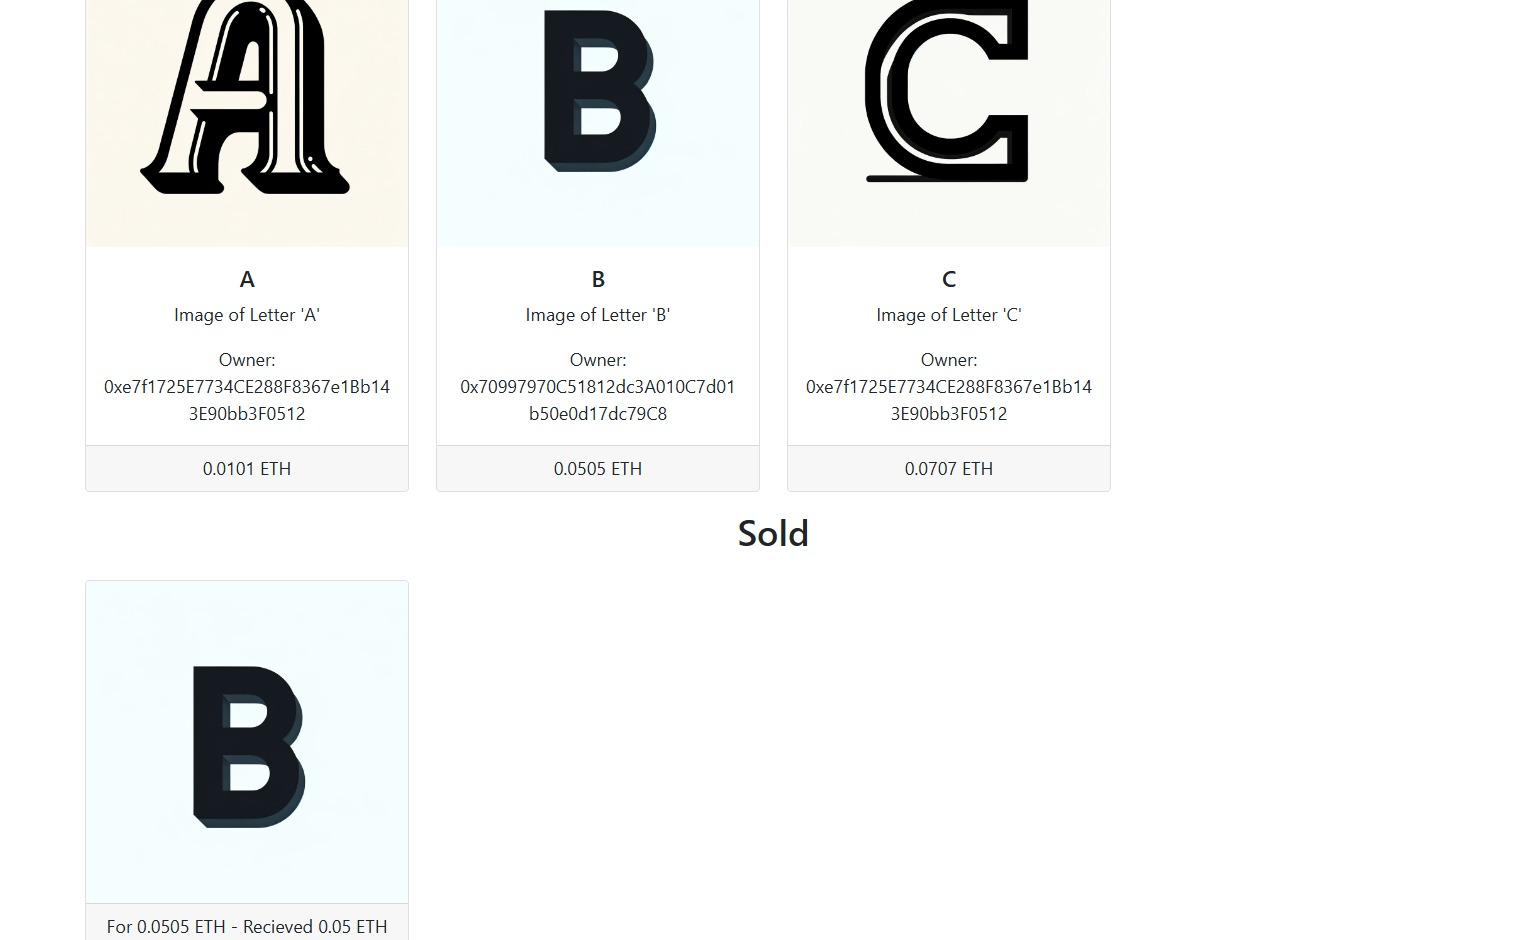
\includegraphics[scale=0.25]{gambar/tampilan_pada_listed_items.jpeg}}
        % Keterangan gambar yang diinputkan
        \caption{Tampilan \emph{Listed items} ketika melakukan pembelian}
        % Label referensi dari gambar yang diinputkan
        \label{fig:new_listed_item}
        \end{figure}

      \item Pada gambar \ref{fig:new_listed_item} di atas, tampilan menunjukkan NFT 'B' yang telah berhasil dibeli oleh pengguna dari akun kedua, sebagaimana terlihat dari pergantian address pemilik ('Owner') pada NFT tersebut dari \emph{address} akun 1 ke alamat \emph{address} dari akun 2. Proses pembelian NFT ini diawali ketika pengguna mengklik tombol pembelian pada salah satu item NFT yang terdaftar di halaman utama, yang kemudian memicu interaksi dengan MetaMask wallet. Pengguna kemudian diminta untuk mengonfirmasi dan menyelesaikan pembayaran melalui wallet tersebut. Setelah transaksi berhasil diverifikasi dan konfirmasi pembayaran diterima, sistem otomatis mengubah status item di halaman "My Listed Items" menjadi "Sold", yang menandakan bahwa item tersebut telah sukses terjual dan tidak lagi tersedia untuk pembelian oleh pengguna lain. Perubahan status ini tidak hanya memastikan transparansi dalam status ketersediaan NFT tetapi juga menunjukkan pembaruan real-time dari kepemilikan aset di platform.
      
      \item Pada gambar \ref{fig:new_listed_item} juga setelah pengguna berhasil menyelesaikan pembelian NFT dari halaman utama, sistem akan memperbarui status NFT tersebut di halaman "My Listed Items" untuk menunjukkan bahwa item telah terjual. Bagian "Sold" di halaman ini akan menampilkan NFT yang telah dibeli, memberikan informasi bahwa NFT tersebut tidak lagi tersedia untuk dibeli oleh pengguna lain. Tampilan ini mencakup gambar NFT, harga jual, serta indikasi bahwa transaksi telah berhasil dengan menunjukkan jumlah ETH yang diterima. Proses ini memastikan bahwa semua pengguna aplikasi dapat melihat secara jelas item yang telah terjual, meningkatkan transparansi dan memudahkan pelacakan kepemilikan NFT. Fungsi ini sangat penting dalam ekosistem NFT, di mana verifikasi kepemilikan dan status penjualan harus diperbarui secara real-time untuk mencegah penjualan ganda dan memastikan integritas platform.
    
      \begin{figure} [H] \centering
        % Nama dari file gambar yang diinputkan
        \frame{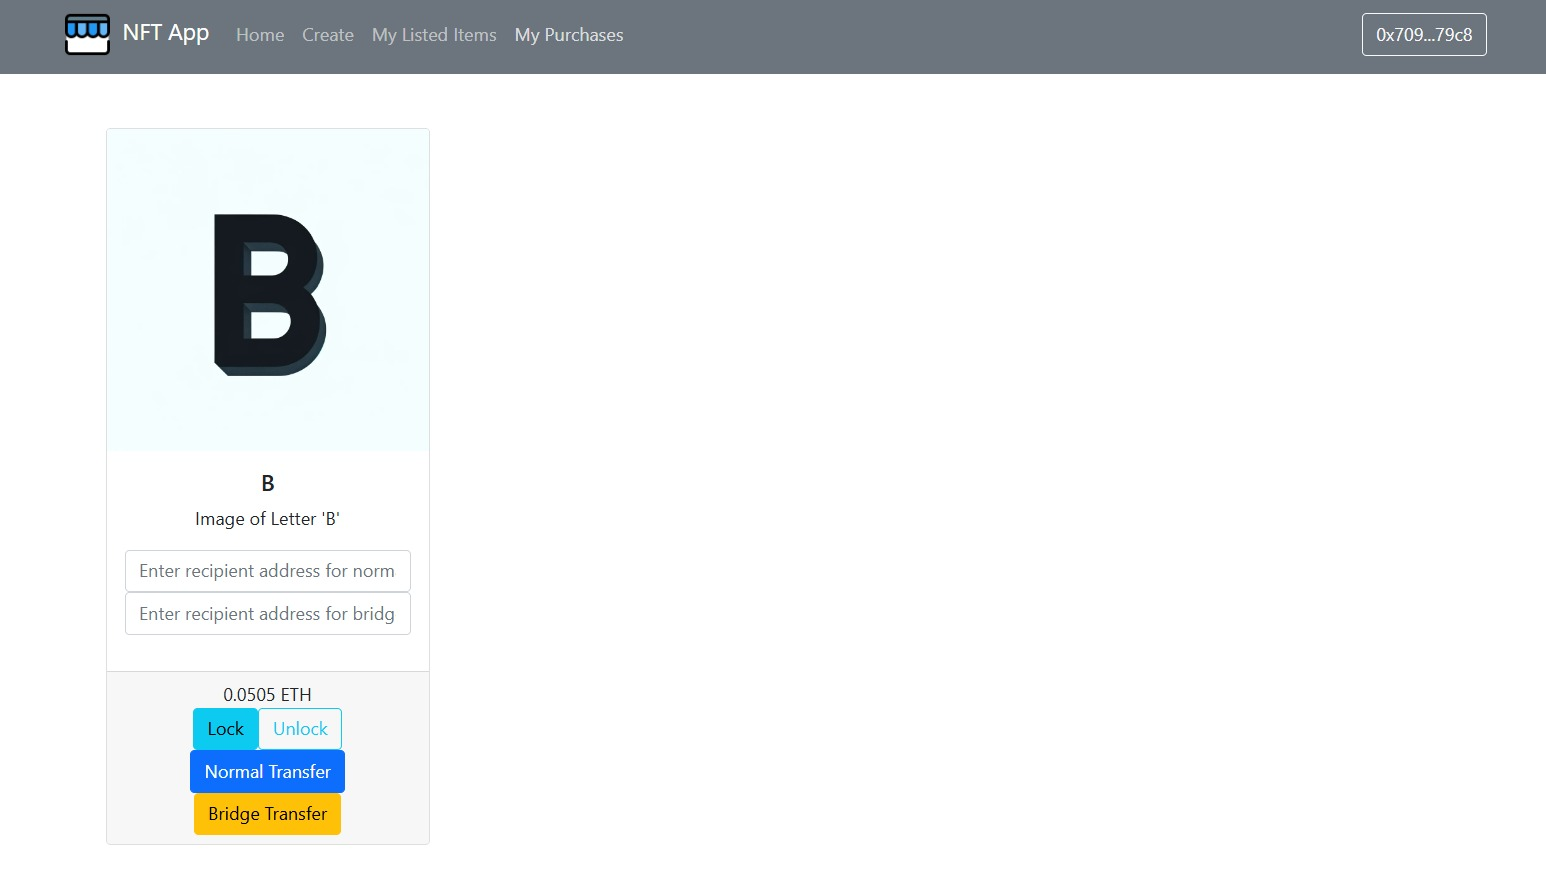
\includegraphics[scale=0.25]{gambar/my_purchases_akun2.jpg}}
        % Keterangan gambar yang diinputkan
        \caption{Tampilan halaman \emph{my purchases} ketika sudah melakukan pembelian}
        % Label referensi dari gambar yang diinputkan
        \label{fig:my_purchases}
        \end{figure}
        \item Lalu pada gambar \ref{fig:my_purchases} adalah tampilan dari halaman \emph{my purchases} di address akun kedua. Pada tampilan ini pemilik dari NFT dapat melihat dari koleksi NFT yang telah dibeli dan juga NFT yang telah dibeli dapat dilakukan hal yaitu \emph{transfer ownership}. \emph{Transfer ownership} yang dapat dilakukan ada dua hal, yaitu \emph{transfer} pada \emph{network} atau \emph{blockchain} yang sama dan juga ada \emph{transfer} pada \emph{network} atau \emph{blockchain} yang berbeda. Kedua fungsi tersebut berbeda karena untuk lintas \emph{blockchain} diperlukan beberapa tahapan atau protokol yaitu terdapat protokol \emph{lock} dan \emph{unlock}. Pada tahapan selanjutnya yang akan dilakukan adalah bagaimana cara melakukan \emph{transfer} dalam satu network yang sama.
        
      \end{itemize}
      
\newpage
\subsection{Pengujian Fitur Transfer \emph{Ownership} Secara \emph{Localhost} Dan Secara Lintas \emph{Blockchain}}

\begin{figure} [H] \centering
  % Nama dari file gambar yang diinputkan
  \frame{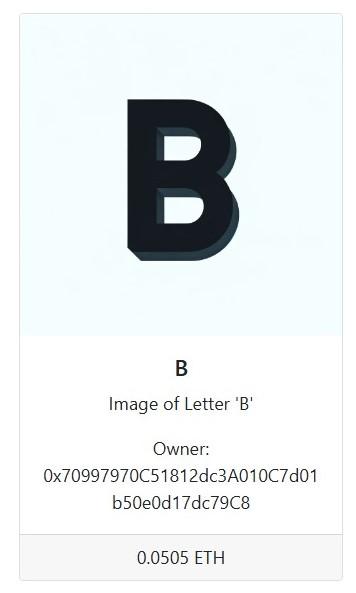
\includegraphics[scale=0.8]{gambar/address_akun_kedua_nft_b.jpeg}}
  % Keterangan gambar yang diinputkan
  \caption{Tampilan halaman \emph{my purchases} ketika sudah melakukan pembelian}
  % Label referensi dari gambar yang diinputkan
  \label{fig:address_nft_b_1}
  \end{figure}

Sebelum melakukan pengujian pemindahan kepemilikan NFT, penggunaan akun ketiga dengan \emph{address} "0x3C44CdDdB6a900fa2b585dd299e03d12FA4293BC" sangat krusial. Akun ini secara khusus disiapkan untuk menangani proses transfer kepemilikan NFT dari akun kedua. Seperti yang terlihat pada gambar \ref*{fig:listeditem}, awalnya NFT diunggah melalui halaman \emph{create} dan secara otomatis, \emph{owner} pertama NFT adalah \emph{address} dari \emph{smart contract} yang melakukan \emph{minting}. Hal ini berubah setelah NFT dibeli, sebagaimana ditunjukkan dalam gambar \ref{fig:address_nft_b_1} di mana \emph{address} akun kedua menjadi pemilik baru. Perpindahan kepemilikan ini terjadi melalui transaksi yang tercatat dan diverifikasi dalam blockchain, memastikan bahwa NFT berpindah tangan dari akun pencipta ke pembeli dengan aman dan terdokumentasi dengan jelas, menunjukkan kekuatan dan fleksibilitas teknologi \emph{smart contract} dalam mengelola aset digital dalam ekosistem blockchain.

\begin{figure} [H] \centering
  % Nama dari file gambar yang diinputkan
  \frame{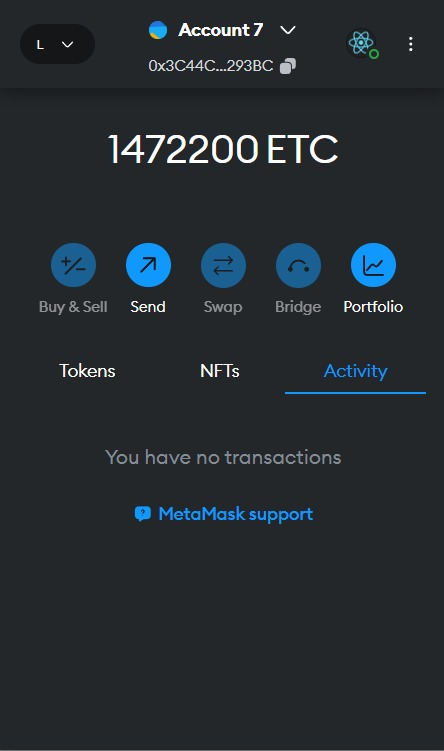
\includegraphics[scale=0.4]{gambar/metamask_akun_3.jpg}}
  % Keterangan gambar yang diinputkan
  \caption{Detail akun ketiga pada Metamask Wallet}
  % Label referensi dari gambar yang diinputkan
  \label{fig:detail_akun_3}
  \end{figure}

Pada gambar \ref*{fig:detail_akun_3}, terlihat tampilan akun MetaMask yang disebut "Account 7" dengan saldo yang menonjol sebanyak 1472200 ETC, yang menunjukkan jumlah Ethereum Classic di dalam wallet. Akun ini, yang beralamat di 0x3C44CdDdB6a900fa2b585dd299e03d12FA4293
BC, belum memiliki catatan transaksi apapun, menandakan bahwa belum ada aktivitas jual beli, pengiriman, penukaran, atau transaksi lainnya yang dilakukan. Hal ini juga memperlihatkan bahwa akun ini adalah akun baru atau belum digunakan untuk transaksi. Akun ini didapatkan dari kunci privat yang berasal dari node Hardhat, sering digunakan dalam pengembangan dan pengujian smart contract di lingkungan lokal. Akun ini direncanakan akan digunakan sebagai penerima dalam proses transfer kepemilikan NFT, memanfaatkan fasilitas yang disediakan MetaMask untuk mengelola aset kripto dan interaksi dengan \emph{blockchain}.

Ekspektasi dari pengujian fitur \emph{transfer ownership} pada web3.0 yang telah dibuat lain adalah sebagai berikut:
\begin{itemize}
    \item Pengguna dari pemilik NFT yang sekarang (pengguna \emph{address} kedua) dapat melakukan pemindahan kepemilikan NFT yang telah dimiliki menjadi kepemilikan pengguna \emph{address} ketiga yang berada dalam \emph{network} yang sama yaitu \emph{localhost}.

    \item Pengguna dari pemilik NFT yang sekarang (pengguna pertama) dapat melakukan pemindahan kepemilikan NFT yang telah dimiliki menjadi kepemilikan pengguna pengguna kedua berada dalam \emph{network} yang berbeda yaitu \emph{Sepolia Testnet} pada pengguna pertama dan \emph{BNB Chain Testnet} pada pengguna kedua.

    \item Pada halaman \emph{my listed item} pembuat dar NFT awal (pengguna \emph{address} pertama) \emph{owner} dari NFT yang telah dilakukan \emph{transfer ownership} secara \emph{localhost} maupun lintas \emph{blockchain} itu alamatnya berganti dari \emph{address} pemilik lama menjadi \emph{address} pemilik baru. 
    
\end{itemize}

Berikut ini merupakan langkah pengujian beserta dengan pembahasan dari pengujian fitur transfer \emph{ownership} Secara \emph{Localhost} Dan Secara Lintas \emph{Blockchain}:

\begin{itemize}
  \item Pada gambar \ref*{fig:my_purchases}, dapat dilihat pada halaman \emph{my purchases} milik \emph{address} akun kedua terdapat NFT "B".  Setelah transaksi pembelian NFT ini, platform menyediakan opsi untuk mengelola NFT tersebut, termasuk kemampuan untuk melakukan transfer kepemilikan atau memblokirnya untuk transaksi lebih lanjut. Pengguna dapat memasukkan alamat penerima untuk transfer normal atau transfer lintas rantai, memanfaatkan fungsionalitas yang memudahkan transfer NFT antara berbagai blockchain atau dalam jaringan yang sama.
  
  \begin{figure} [H] \centering
    % Nama dari file gambar yang diinputkan
    \frame{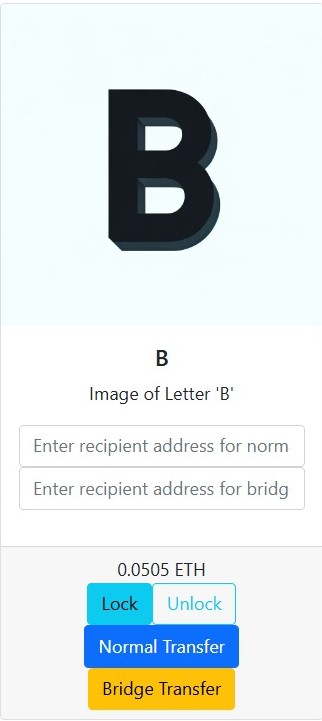
\includegraphics[scale=0.6]{gambar/normal_transfer.jpg}}
    % Keterangan gambar yang diinputkan
    \caption{Tampilan NFT yang siap dilakukan pindah kepemilikan}
    % Label referensi dari gambar yang diinputkan
    \label{fig:normal_transfer}
    \end{figure}

  \item Pada pengujian ini, digunakan NFT "B" yang akan dilakukan transfer \emph{ownership} dalam satu \emph{network}, pada kolom pertama yang bertuliskan "Enter recipient address for normal transfer \emph{ownership}" akan dimasukkan \emph{address} dari akun ketiga yang berupa "\emph{0x3C44CdD dB6a900fa2b585dd299e03d12FA4293BC}". Setelah dimasukkan \emph{address} tersebut maka akan langsung saja ditekannya tombol "\emph{Normal Transfer}". Tombol "\emph{Normal Transfer}" tersebut lalu akan membuat pengguna langsung membuka window dari Metamask Wallet untuk melakukan transaksi pembayaran dari "\emph{gas}" atau fee yang harus dibayarkan setiap kali kode dari \emph{smart contract} tereksekusi. Setiap aksi yang dilakukan oleh \emph{smart contract} seperti transaksi, perubahan data, atau eksekusi fungsi—memerlukan gas tertentu.
  
  \begin{figure} [H] \centering
  % Nama dari file gambar yang diinputkan
  \frame{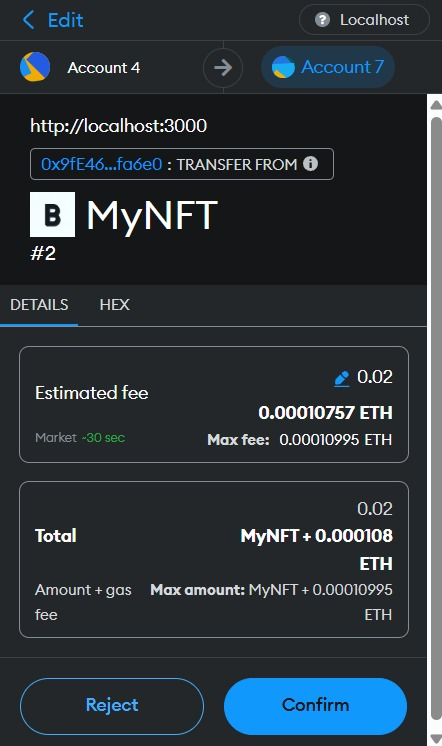
\includegraphics[scale=0.45]{gambar/my_nft_b.jpg}}
  % Keterangan gambar yang diinputkan
  \caption{Tampilan NFT yang siap dilakukan pindah kepemilikan}
  % Label referensi dari gambar yang diinputkan
  \label{fig:nft_b}
  \end{figure}
  
  \item Gambar \ref*{fig:nft_b} ini menunjukkan tampilan antarmuka Metamask saat pengguna kedua siap melakukan transaksi transfer dari NFT bernama "MyNFT" dengan nomor \#2. Nomor \#2 ditunjukkan bahwa NFT itu memiliki indeks urutan kedua. Pada tampilan ini, pengguna diberi informasi mengenai jumlah ETH yang akan ditransfer sebesar 0.02 ETH dan biaya transaksi yang diperkirakan. Biaya ini terbagi menjadi dua, yaitu biaya perkiraan (estimated fee) sebesar 0.00010757 ETH dan biaya maksimal (\emph{max fee}) sebesar 0.00010995 ETH, yang memberikan kejelasan tentang berapa banyak gas yang mungkin diperlukan untuk menyelesaikan transaksi tersebut dalam waktu kurang lebih 30 detik. Fitur ini memfasilitasi pengguna dalam memastikan bahwa mereka memiliki cukup saldo untuk menutupi biaya transaksi saat melakukan transfer NFT. Tampilan juga menawarkan pilihan untuk menyetujui atau menolak transaksi yang akan dilakukan.
  
  \begin{figure} [H] \centering
  % Nama dari file gambar yang diinputkan
  \frame{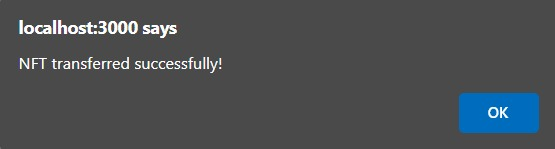
\includegraphics[scale=0.70]{gambar/transfer_berhasil.jpg}}
  % Keterangan gambar yang diinputkan
  \caption{\emph{Alert} "\emph{NFT transferred successfully!}" ketika NFT berhasil dipindahkan}
  % Label referensi dari gambar yang diinputkan
  \label{fig:alert}
  \end{figure}

  \item Setelah pengguna melakukan konfirmasi transaksi pada Metamask Wallet seperti pada gambar \ref*{fig:normal_transfer} dan transaksi berhasil, maka akan muncul \emph{alert} berupa "\emph{NFT transferred successfully!}".
  
  \begin{figure} [H] \centering
    % Nama dari file gambar yang diinputkan
    \frame{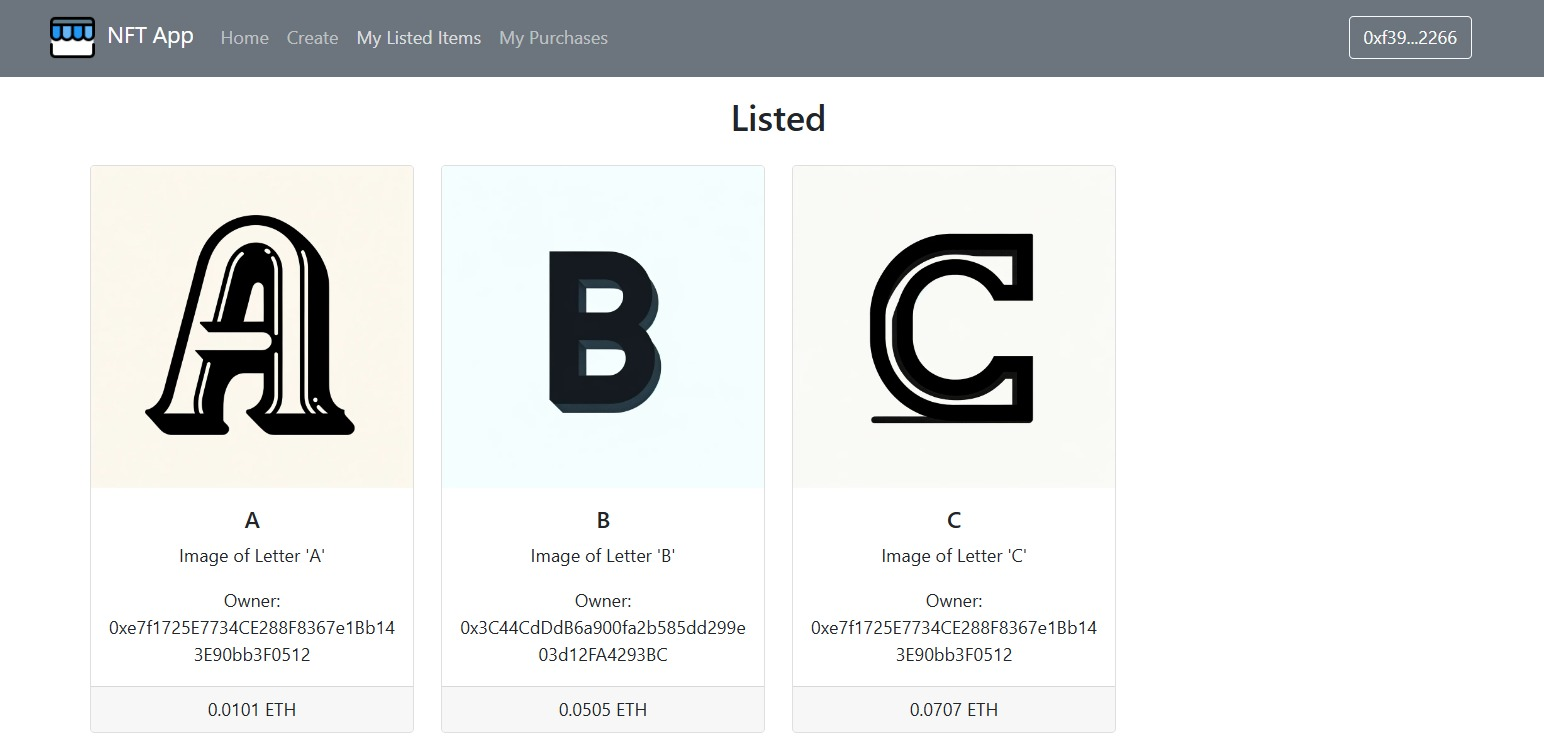
\includegraphics[scale=0.25]{gambar/letter_b_to_akun3.jpg}}
    % Keterangan gambar yang diinputkan
    \caption{\emph{Alert} "\emph{NFT transferred successfully!}" ketika NFT berhasil dipindahkan}
    % Label referensi dari gambar yang diinputkan
    \label{fig:letter_b_akun3}
    \end{figure}

  \item Dapat dilihat pada gambar \ref*{fig:letter_b_akun3} pada halaman \emph{my listed items} milik pengguna \emph{address} pertama yang me-\emph{minting} NFT B, jika dibandingkan dengan gambar \ref*{fig:address_nft_b_1}, \emph{owner} dari NFT B telah berganti menjadi \emph{address} milik akun ketiga. Ini membuktikan bahwa NFT B kepemilikannya berhasil dipindahkan dari \emph{address} pengguna kedua menjadi \emph{address} pengguna ketiga.

  \begin{figure} [H] \centering
    % Nama dari file gambar yang diinputkan
    \frame{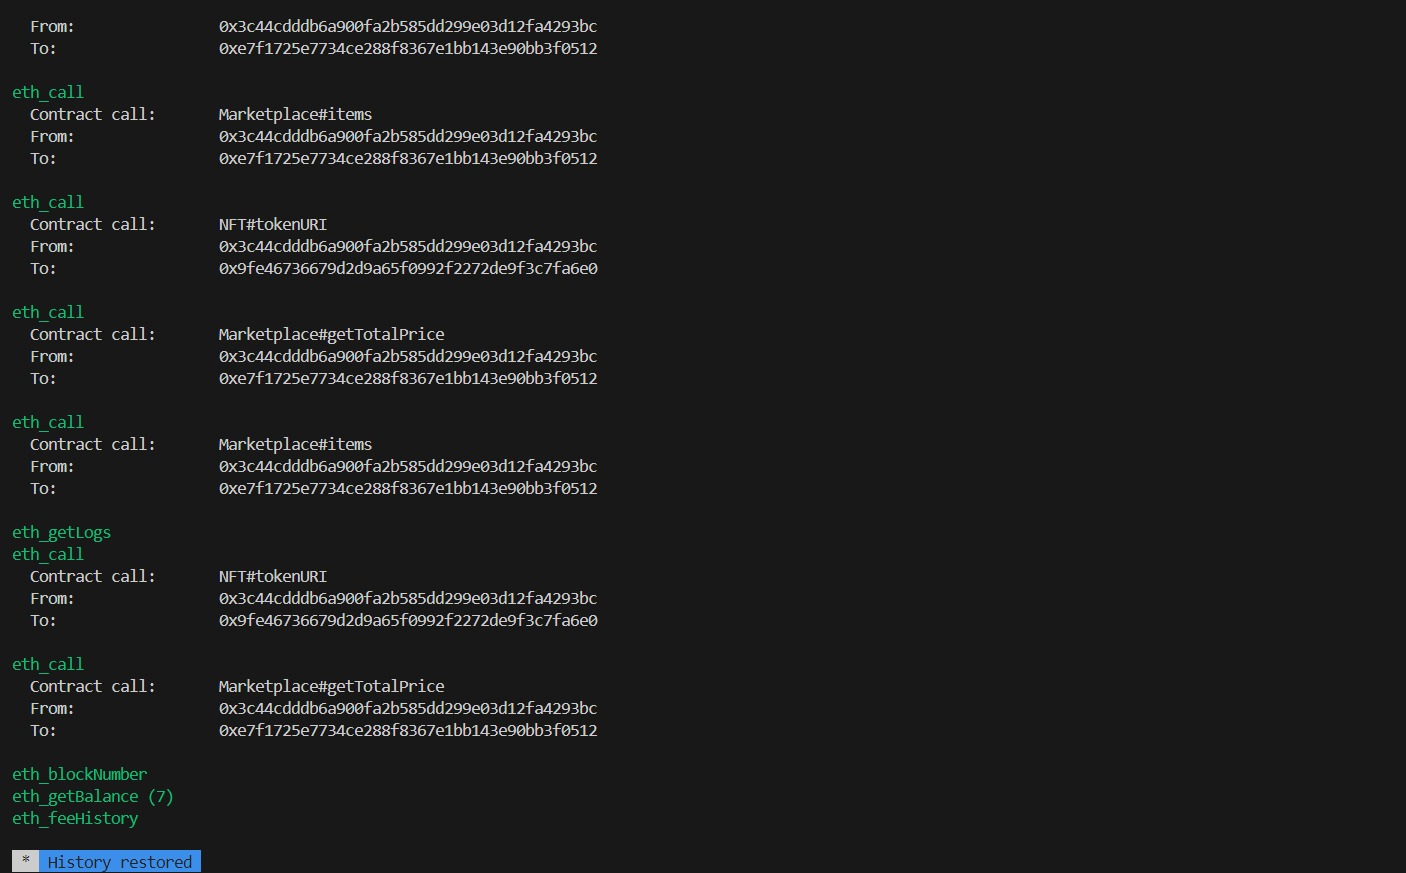
\includegraphics[scale=0.27]{gambar/hardhat_transaction.jpg}}
    % Keterangan gambar yang diinputkan
    \caption{Console Transaksi Pada \emph{Hardhat Node}}
    % Label referensi dari gambar yang diinputkan
    \label{fig:hardhat}
    \end{figure}

    \item Pada gambar \ref*{fig:hardhat} adalah detail transaksi yang terjadi pada \emph{smart contract} ketika ada fungsi yang tersekekusi. Dikarenakan pengembangan web3.0 dan juga sistem \emph{smart contract} ini dilakukan secara lokal, maka \emph{contract call} dan juga detail dari \emph{hash block} hanya dapat dilihat pada \emph{node} yang berada pada EVM milik Hardhat.
    
    \begin{figure} [H] \centering
      % Nama dari file gambar yang diinputkan
      \frame{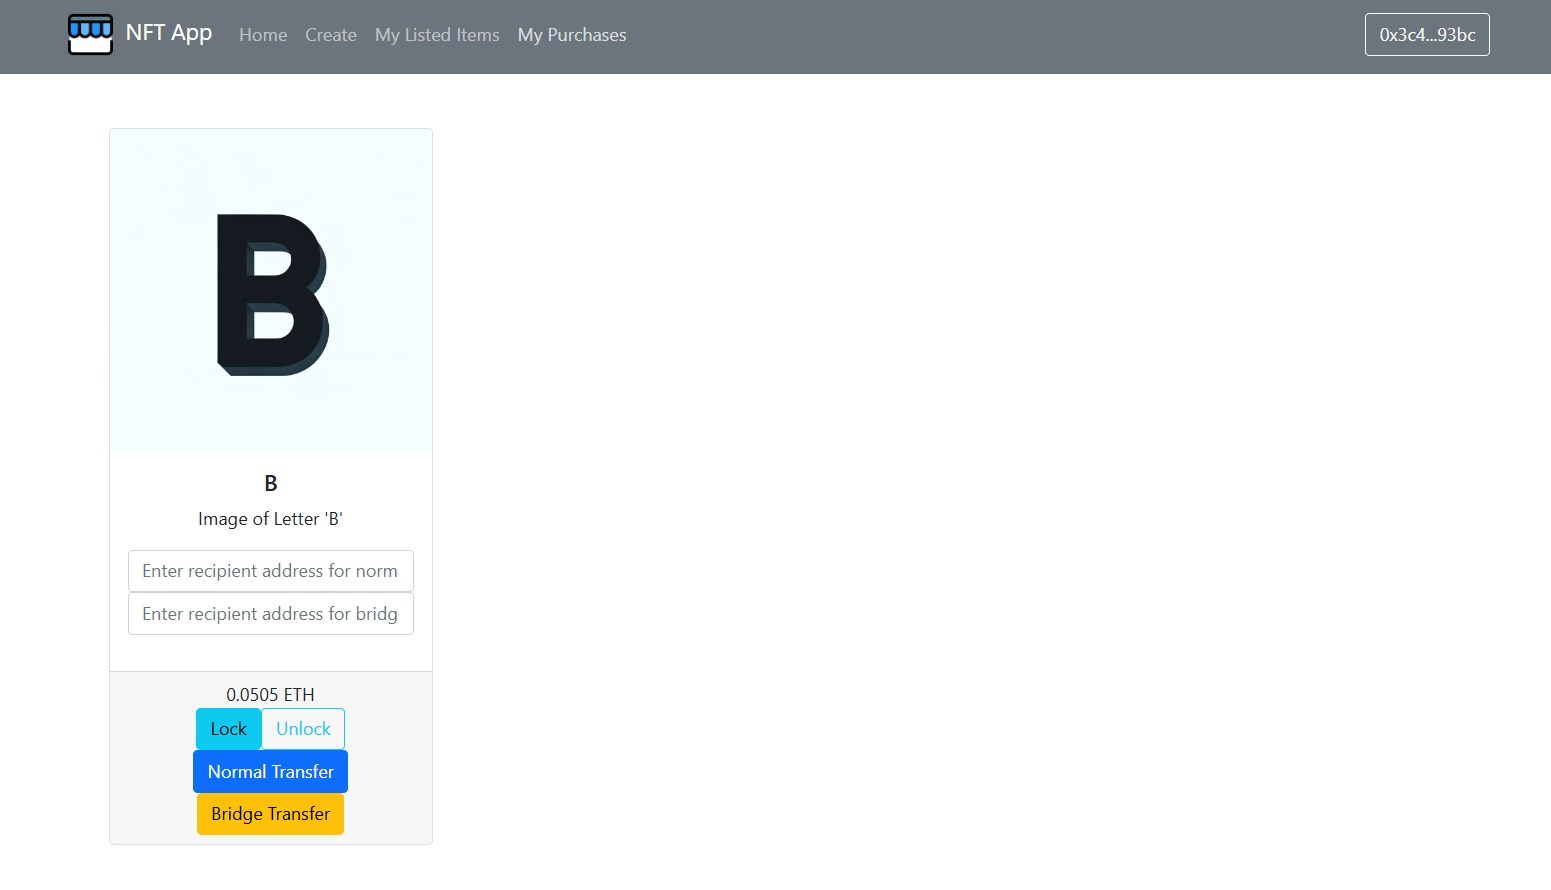
\includegraphics[scale=0.27]{gambar/letter_b_akun3.jpg}}
      % Keterangan gambar yang diinputkan
      \caption{Tampilan halaman \emph{my purchases} pada akun ketiga}
      % Label referensi dari gambar yang diinputkan
      \label{fig:akunketiga}
      \end{figure}

    \item Lalu selain dari \ref*{fig:letter_b_akun3} juga terdapat hasil bahwa NFT telah berpindah pada akun ketiga. Hal ini dapat dilihat pada \emph{box} kanan atas menunjukkan \emph{address} dari akun ketiga yang berarti ini adalah halaman \emph{my purchases} milik akun ketiga. Lalu akun ketiga ini juga yang memiliki wewenang penuh dalam kepemilikan NFT yang sebelumnya dimiliki oleh akun kedua.
    
    \begin{figure} [H] \centering
      \centering
      \begin{subfigure}{0.45\textwidth}
          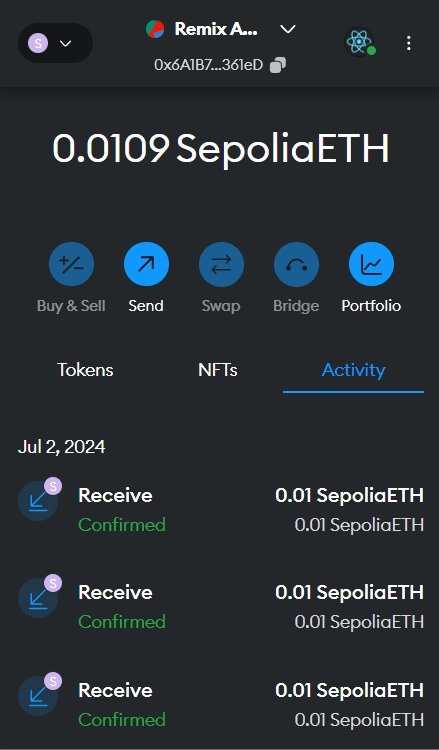
\includegraphics[scale=0.32]{gambar/sepolia_akun.jpg}
          \caption{}
          \label{fig:sepolia}
      \end{subfigure}
      \hspace{5pt}
      \begin{subfigure}{0.45\textwidth}
        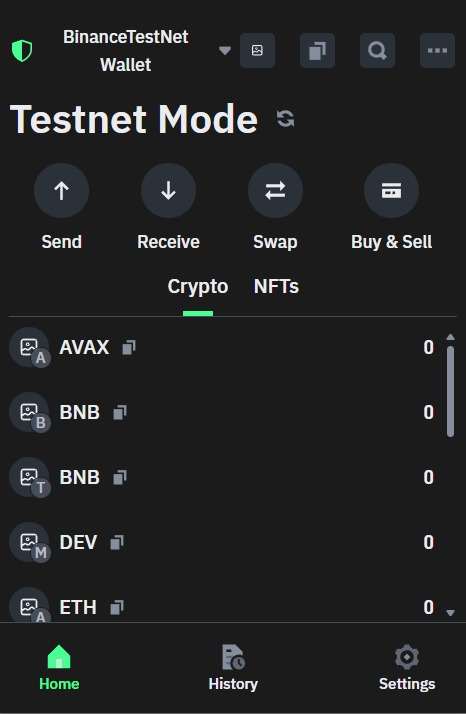
\includegraphics[scale=0.32]{gambar/btc_akun.jpg}
        \caption{}
        \label{fig:binance}
    \end{subfigure}
      \caption{Detail Akun Untuk Pengujian Lintas Rantai}
      \label{fig:detail_akun}
      \end{figure}

    \item Gambar pertama menggambarkan akun di Sepolia Ethereum Testnet dengan saldo SepoliaETH yang ditampilkan secara jelas. Ini termasuk aktivitas terkini yang mencakup penerimaan SepoliaETH, memperlihatkan aktivitas yang dikonfirmasi dalam jaringan. Akun pada gambar pertama ini akan digunakan sebagai \emph{address} penerima dari NFT yang dikirimkan dari \emph{network} yang berbeda. Akun ini memiliki \emph{address} "0x6A1B77e82b61D54C4
    F1A27cd00A27325EBf361eD"
    
    \item Gambar kedua menampilkan BinanceTestNet Wallet dalam mode testnet, yang memungkinkan pengguna untuk mengirim, menerima, bertukar, dan membeli aset kripto seperti AVAX, BNB, DEV, dan ETH dalam lingkungan tes. Akun pada gambar kedua ini akan digunakan sebagai \emph{address} penerima dari NFT yang dikirimkan dari \emph{network} yang berbeda. Akun ini memiliki \emph{address} "0xD066d6576D9485Eb2c2a41BB8B52EcE17a0557d6"
    
    \begin{figure} [H] \centering
      % Nama dari file gambar yang diinputkan
      \frame{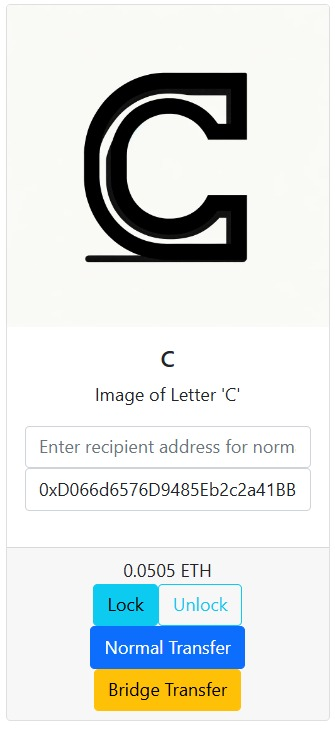
\includegraphics[scale=0.5]{gambar/interoperability_1.jpg}}
      % Keterangan gambar yang diinputkan
      \caption{Memasukkan \emph{address} tujuan untuk \emph{bridge transfer}}
      % Label referensi dari gambar yang diinputkan
      \label{fig:bridge_transfer}
      \end{figure}

    \item Pengujian untuk melakukan tes interoperabilitas atau transfer \emph{ownership} lintas \emph{blockchain} dilakukan dengan prosedur yang terstruktur. Pertama, akun pengirim yang beroperasi di jaringan \emph{localhost} akan memilih NFT yang ingin ditransfer. Kemudian, alamat tujuan dari akun yang berjalan di jaringan Sepolia diisi ke dalam sistem. Proses transfer diawali dengan penguncian (\emph{lock}) NFT untuk memastikan keamanan selama transisi. Fungsi \emph{lock} ini penting untuk mencegah transaksi atau interaksi lain yang mungkin mempengaruhi NFT selama proses transfer belum selesai. Setelah NFT terkunci, barulah transfer ownership akan dijalankan melalui fungsi \emph{bridge transfer}.
    
    \begin{figure} [H] \centering
      % Nama dari file gambar yang diinputkan
      \frame{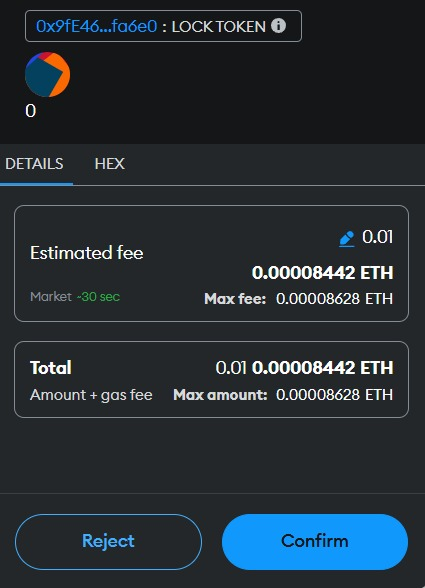
\includegraphics[scale=0.4]{gambar/fungsi_lock.jpg}}
      % Keterangan gambar yang diinputkan
      \caption{Konfirmasi pembayaran gas dari fungsi \emph{lock token} di Metamask Wallet}
      % Label referensi dari gambar yang diinputkan
      \label{fig:lock_token}
      \end{figure}
    
    \item Setelah melakukan konfirmasi pembayaran gas dari fungsi \emph{lock} token, kondisi NFT berubah menjadi \emph{locked}. Setelah NFT menjadi \emph{locked} maka NFT sudah aman untuk dilakukan transaksi lintas \emph{blockchain}. 
    
    \begin{figure} [H] \centering
      % Nama dari file gambar yang diinputkan
      \frame{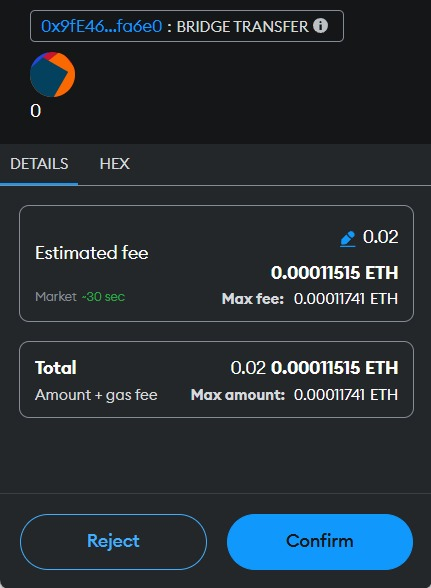
\includegraphics[scale=0.4]{gambar/bridge.jpg}}
      % Keterangan gambar yang diinputkan
      \caption{Konfirmasi pembayaran gas dari fungsi \emph{bridge} transfer di Metamask Wallet}
      % Label referensi dari gambar yang diinputkan
      \label{fig:bridge_transfer}
      \end{figure}
    
      \item Setelah melakukan konfirmasi pembayaran gas dari fungsi \emph{bridge} transfer, kepemilikan dari NFT "C" berpindah dari akun pertama yang memiliki \emph{address} "0xf39Fd6e51aad88F6
      F4ce6aB8827279cffFb92266" yang berjalan pada \emph{network localhost} menjadi kepemilikan akun yang berjalan pada \emph{network BNB Smart Chain} dengan alamat "0xD066d657
      6D9485Eb2c2a41BB8B52EcE17a0557d6". Hal ini dapat dibuktikan pada gambar di bawah ini.

      \begin{figure} [H] \centering
        % Nama dari file gambar yang diinputkan
        \frame{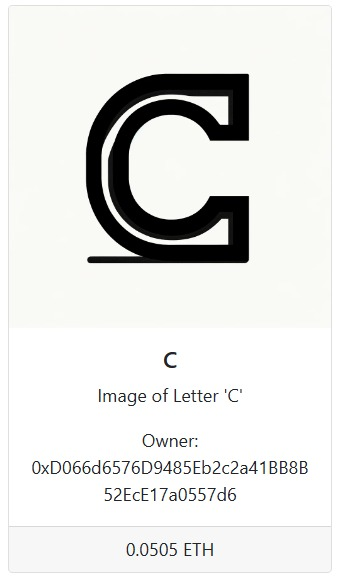
\includegraphics[scale=0.45]{gambar/smart_chain.jpg}}
        % Keterangan gambar yang diinputkan
        \caption{Kepemilikan NFT "C" Berganti Menjadi Akun \emph{Network BNB Smart Chain}}
        % Label referensi dari gambar yang diinputkan
        \label{fig:bridge_transfer}
        \end{figure}
      
      \item Kemudian hal yang perlu dilakukan yang terakhir adalah mengubah \emph{state} dari NFT tersebut yang awalnya "\emph{locked}" menjadi "\emph{unlocked}". Hal ini harus dilakukan agar NFT tersebut dapat digunakan untuk transaksi lagi pada \emph{network} tersebut.
      
      \begin{figure} [H] \centering
        % Nama dari file gambar yang diinputkan
        \frame{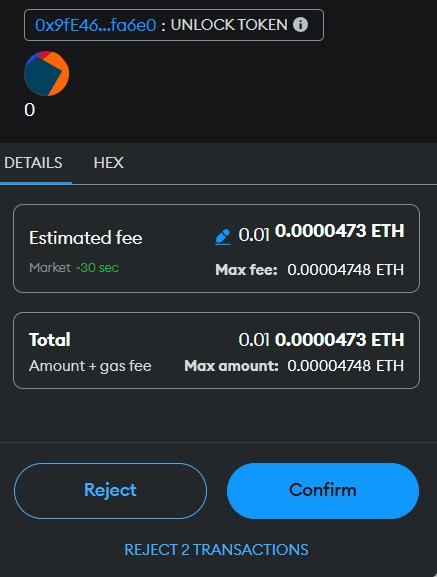
\includegraphics[scale=0.4]{gambar/unlock_token.jpg}}
        % Keterangan gambar yang diinputkan
        \caption{Konfirmasi Pembayaran Gas \emph{Unlock} Token}
        % Label referensi dari gambar yang diinputkan
        \label{fig:unlock_token}
        \end{figure}
      
    \item Setelah melakukan penguncian NFT, langkah berikutnya adalah membuka kunci atau "unlock" NFT tersebut agar dapat kembali digunakan dalam transaksi. Proses ini melibatkan interaksi dengan sistem \emph{blockchain} yang tercatat sebagai transaksi dengan estimasi biaya yang diperlihatkan dalam gambar. Di sini, biaya transaksi atau '\emph{gas fee}' yang diperkirakan untuk membuka kunci token ditampilkan, menekankan pentingnya memperhatikan biaya transaksi yang harus dibayar untuk memproses kegiatan ini di \emph{blockchain}. Proses membuka kunci ini tidak hanya mengizinkan pemilik untuk memindahkan atau menjual NFT tersebut, tetapi juga penting untuk memastikan fleksibilitas dan likuiditas NFT di pasar.
    
    \begin{figure} [H] \centering
    % Nama dari file gambar yang diinputkan
    \frame{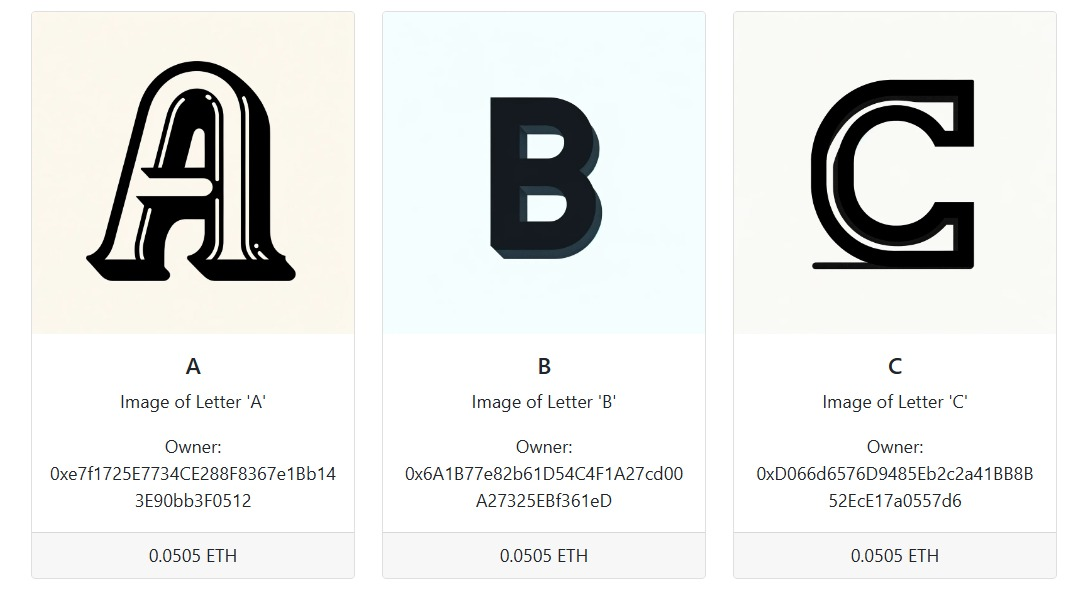
\includegraphics[scale=0.4]{gambar/interoperabilitas_2.jpg}}
    % Keterangan gambar yang diinputkan
    \caption{Hasil Akhir Dari Transfer Lintas Rantai}
    % Label referensi dari gambar yang diinputkan
    \label{fig:lintas_rantai}
    \end{figure}

    \item Setelah dilakukan pengujian yang sama tetapi memasukkan \emph{address} dari akun yang berada pada \emph{network sepolia ethereum}, untuk transfer \emph{ownership} NFT B dapat dilihat di gambar \ref*{fig:lintas_rantai} kepemilikan atau \emph{owner} dari NFT B juga berubah menjadi \emph{address} dari akun \emph{sepolia}. 
    
    \begin{figure} [H] \centering
      % Nama dari file gambar yang diinputkan
      \frame{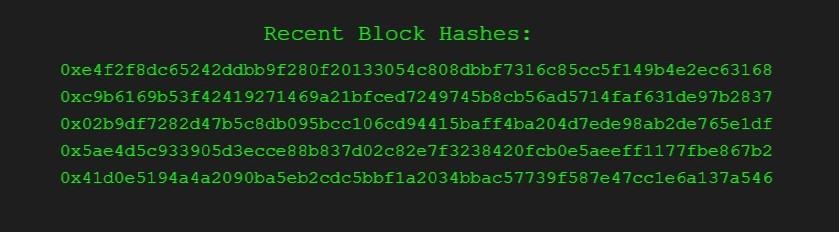
\includegraphics[scale=0.7]{gambar/block_hash.jpg}}
      % Keterangan gambar yang diinputkan
      \caption{\emph{Block Hash} dari setiap transaksi}
      % Label referensi dari gambar yang diinputkan
      \label{fig:hash_block}
      \end{figure}

    \item Pada gambar \ref*{fig:hash_block}, merupakan \emph{block hash} dari transaksi yang telah terjadi. \emph{Hash Blocks} ini didapatkan dari Hardhat. \emph{Block hash} adalah nilai unik yang dihasilkan dari \emph{blok} data dalam \emph{blockchain}, yang bertindak sebagai identitas digital \emph{blok} tersebut. Hash ini dihasilkan menggunakan algoritma hash kriptografi, yang mengubah informasi \emph{blok} menjadi string karakter tetap panjang yang kompleks dan unik. Proses ini memastikan keamanan dan integritas data dalam \emph{blockchain} karena setiap perubahan kecil pada \emph{blok} akan menghasilkan hash yang sangat berbeda, sehingga mudah untuk mendeteksi perubahan atau manipulasi data. Hash \emph{blok} juga digunakan untuk menghubungkan \emph{blok}-\emph{blok} dalam \emph{blockchain} \emph{hash} dari \emph{blok} sebelumnya dimasukkan ke dalam \emph{blok} berikutnya, menciptakan rantai data yang terkait dan aman.
\end{itemize}